
\chapter{STATE OF ART ANALYSIS AND SYNTHESIS OF SYMMETRIC CRYPTOGRAPHIC TRANSFORMATIONS}
\label{sec:symmetry_review}

Evaluation and design rationale are essential parts of developing and
deploying  the considered cryptographic security system. The primary goal of
cryptography is to design mathematical methods for providing security against
adversary's malicious actions under any predetermined conditions.

However, as practice shows, it's unfeasible to take into account all possible
attacks that may be invented in the future due to technological and scientific
innovations during the development stage. Therefore, the most efficient known
method for analysing computationally strong cryptographic primitives is
complexity evaluation of every known applicable attack.

\section{Classification of attacks on symmetric ciphers}

Attacks on symmetric ciphers are defined by the abilities and data
that an adversary can operate with. Most of them refer actions that may be
done to cipher entities such as plaintexts and ciphertexts, however a separate
class of attacks that exploits cipher implementation rather than the
algorithm itself exists.

A ciphertext-only attack leaves the adversary with a set of ciphertexts that
she\footnote{Following the tradition started by Shafi Goldwasser in her Lecture
Notes on Cryptography, ``she'' is used throughout the text as referring to a
subject of unknown gender.} can use to recover the corresponding
plaintext or encryption key. Such conditions are the most complex for
cryptanalyst. In a known plaintext attack the adversary has a fixed set of
plaintext and ciphertext pairs~\cite{menezes:applied_cryptography}.

In chosen plaintext and chosen ciphertext attacks the adversary gets an
ability to encrypt plaintexts or decrypt ciphertexts of her choice
respectively. So the cipher needs to have such plaintext and ciphertext
spaces that would make it infeasible for the attacker to get full dictionary of
all possible plaintexts and corresponding
ciphertexts~\cite{menezes:applied_cryptography}. 

Related key attacks exploits possible relations between encryption keys to
break the cryptographic system~\cite{StampLow:AppliedCryptanalysis}.

Side channel attacks are somewhat outside of mathematical attacks scope. They
use some cipher implementation peculiarities to gain information about the
encryption key observing the cryptographic system during operation. So far no
mathematical countermeasures exist that would guarantee the security of the
transformation against these types of attacks ~\cite{Quisquater:sidechannel}.

A cipher is considered to be insecure if any type of attack exists that allows
to get some information about the key with a complexity lower than a brute
force. 

\section{Block ciphers}

A block cipher is a function which maps $n$-bit plaintext blocks to $n$-bit 
ciphertext blocks, parameterized by a $k$-bit key
$K$~\cite{menezes:applied_cryptography}. Here $n$ is called the blocklength.
The encryption key $K$ has to be random. In order to always provide unique and
correct decryption the mapping function defined by a chosen key must be
bijective.

A straightforward usage of a block cipher to encrypt separate blocks of data may have
disadvantage in many applications. Consequently, several block cipher modes of
operations have been developed to satisfy various security purposes.

\subsection{Algebraic representation}
\label{sec:block-algebraic}

A symmetric block cipher may be represented as an algebraic
system~\cite{babash:cryptography}
\begin{equation}
\label{eqn:block-algebraic}
\Sigma_{A} = \left< X, K, Y, E, D \right> \enspace, 
\end{equation}
where $X$ is a plaintext space defined over finite alphabet $Q_X$, \\ 
$K$ --- a key set (usually defined by fixed length strings over $Q_X$), \\
$Y$ --- ciphertext space defined over finite alphabet $Q_Y$, \\
$E: X \times K \rightarrow Y$ --- a set of enciphering rules based on
parametrized maps $e_k(x) = y$ for which $k \in K$, $x \in X$, $y \in Y$. \\
Mappings $e_k(\cdot)$ and $d_k(\cdot)$ for any $k \in K$  are bijective and
ensure satisfaction of both conditions $d_k(e_k(x)) = x$ and $e_k(d_k(y)) = y$.

Plaintext and ciphertext spaces of all widespread modern symmetric ciphers 
coincide ($Q_X = Q_Y$), so such ciphers are therefore endomorphic, that is 
\mbox{$X = Y$}.

For cryptographically secure ciphers the sets of encrypting and decrypting
rules must have random mapping properties, and $e_k(\cdot)$, $d_k(\cdot)$ must
be random permutations.


\subsection{Modes of operation}

Simple encryption of data chunks block-by-block is called a electronics
codebook mode (ECB). As seen from figure~\ref{fig:mode-ecb} each plaintext is
encrypted independently. Error propagation is limited within one block, but
this mode is insecure for encryption large correlated
data~\cite{menezes:applied_cryptography}.
\begin{figure}[htbp]
	\centering
	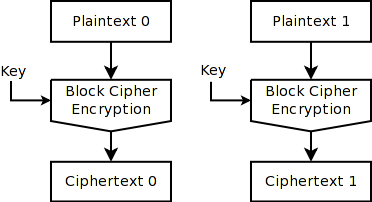
\includegraphics[scale=0.6]{modes_ecb}
	\caption{ECB mode of operation}
	\label{fig:mode-ecb}
\end{figure}

Cipher block chaining mode (CBC) is represented on figure~\ref{fig:mode-cbc}.
In CBC mode two identical plaintext do not encrypt to the same ciphertext as
the encryption depend on the initialization vector (IV) and two previous blocks
instead. This causes error propagation in ciphertext expand to two blocks, but
modifications to plaintext influence all subsequent blocks and make correct
decryption impossible. Such encryption mode is also more secure for enciphering
correlated data~\cite{menezes:applied_cryptography}.

Cipher feedback mode (CFB) shown on figure~\ref{fig:mode-cfb} turns a block
cipher into self-synchronizing (see \ref{sec:stream_ciphers_classification})
stream cipher. 
\begin{figure}[htbp]
	\centering
	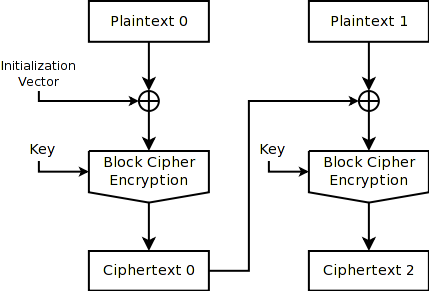
\includegraphics[scale=0.6]{modes_cbc}
	\caption{CBC mode of operation}
	\label{fig:mode-cbc}
\end{figure}
\begin{figure}[htbp]
	\centering
	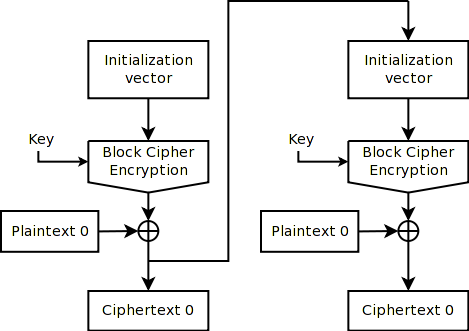
\includegraphics[scale=0.6]{modes_cfb}
	\caption{CFB mode of operation}
	\label{fig:mode-cfb}
\end{figure}

Output feedback mode (OFB) is similar to CFB (figure~\ref{fig:mode-ofb}) and
differs only by a feedback connection.
\begin{figure}[htbp]
	\centering
	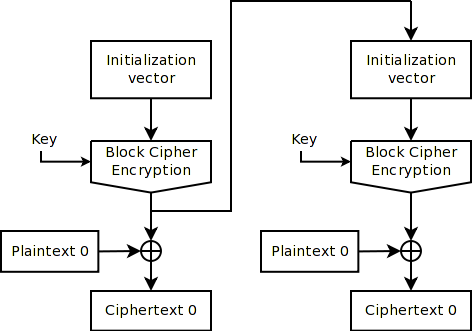
\includegraphics[scale=0.6]{modes_ofb}
	\caption{OFB mode of operation}
	\label{fig:mode-ofb}
\end{figure}
The main advantages of this mode is
absence of error propagation (since keystream generation doesn't depend on the
plaintext) and parallel processing capability.

\clearpage
\section{Stream ciphers}

The distinct difference between stream ciphers and block ciphers was for the
first time defined by Rainer Rueppel~\cite{robshaw:rsa:streamciphers}: 
\begin{quote}
    ``Block ciphers operate with a fixed transformation on large blocks of
    plaintext data; stream ciphers operate with a time-varying transformation on
    individual plaintext digits''.
\end{quote}
Stream ciphers gained great progress since Shannon's analysis of the 
Vernam cipher where he proved it to be theoretically
unbreakable~\cite{shannon:secrecy}. However such cryptosystem were
complex and unprofitable to implement because of the need of secret channel to exchange key
material which was the size of the message itself.

Trying to overcome disadvantages of the Vernam cryptosystem stream ciphers
inherit the idea, but use short key instead to generate a pseudo-random sequence
of needed length. That is, plaintext is encrypted into ciphertext with
pseudo-random sequence,  called the keystream, which is produced by a finite
state automaton whose initial state is determined by a secret key. Therefore
stream ciphers require high structural secrecy in order to be cryptographically
strong.

Stream ciphers are fast and well suited for hardware though some
cryptoalgorithms designed for efficient software implementation exist. They are
used in cases of continuous or unknown amount of data to be encrypted, strict
buffering constraints.

\subsection{Classification}
\label{sec:stream_ciphers_classification}

Depending on the choice of how the next state of cryptosystem is generated from
the current state, two types of stream ciphers are distinguished: synchronous
and self-synchronizing (or asynchronous)~\cite{menezes:applied_cryptography}.

In synchronous stream ciphers the next state of the automaton is independent of
plaintext and ciphertext. Such ciphers have no error-propagation and
consequently don't detect errors during decryption. This fact allows an attacker
to inconspicuously alter ciphertext which will be successfully decrypted to a
different plaintext. Another significance lies in the fact that encrypting and
decrypting devices must constantly stay synchronized. Otherwise the decryption
will fail. 

Asynchronous stream ciphers are able to resume correct decryption in case
transmitter and receiver fall unsynchronized. Error-propagation is limited to
the state bits that depend on previously generated ciphertexts. Such ciphers are
difficult for analysis because the keystream depends on input message. They
are also vulnerable to playback attack: if an attacker repeats some previously
recorded ciphertext, the receiver will successfully decrypt it (after
synchronization) and consider the message to be valid unless time markers are
used.

\subsection{Design principles}

Rainer Rueppel distinguished four approaches to stream cipher
construction~\cite{schneier:applied_cryptography:2}:
\begin{enumerate}
    \item system-theoretic approach; use fundamental design principles to create
        difficult and unknown problem for the cryptanalyst;
    \item information-theoretic approach; try to keep the cryptanalyst in the
        dark about the plaintext; she will never get a unique solution;
    \item complexity-theoretic approach; make the cryptosystem equivalent to
        some known and difficult problem (factorization, taking discrete
        logarithms);
    \item randomized approach; generate unsolvable problem by forcing the
        cryptanalyst to examine lots of useless data.
\end{enumerate}
Engineering and analysing of numerous stream ciphers resulted in essential
design criteria~\cite{rueppel1986analysis}:
\begin{enumerate}
    \item long period;
    \item linear complexity;
    \item statistical criteria;
    \item confusion --- every keystream bit must be a complex transformation of
        all the key bits;
    \item diffusion --- redundancies in substructures must be dissipated into
        long-range statistics;
    \item nonlinearity criteria for Boolean functions.
\end{enumerate}
However it is impossible to prove such cryptosystems are secure enough. A cipher
might satisfy all criteria and still be weak to some cryptanalysis techniques.

\subsubsection{Feedback shift registers}

Any feedback shift register consists of a shift register and a feedback
function~\cite{schneier:applied_cryptography:2}. The shift register itself is a
sequence of bits. New pseudo-random bit is generated by shifting the sequence
one bit to the right. The new input bit of the register is computed as a
function of some bits already in register.

Linear feedback shift register (LFSR) is widely used in stream ciphers. Its
feedback function is XOR of some bits in register (see Figure
\ref{fig:lfsr-fib}).  The list of such bits is called a tap sequence. Such type
of LFSR is called a Fibonacci configuration. A $n$-bit LFSR is able to produce a
pseudo-random sequence of period $2^n - 1$ bits. In order to get a
maximal-period linear sequence ($m$-sequence), the tap sequence must be formed
by a primitive polynomial modulo 2. Even though using sparse polynomials leads
to more efficient software implementation, dense polynomials are better for
cryptographic applications. The only secret parameter of LFSR should be the
initial state derived from the master key.
\begin{figure}[htbp]
    \centering
    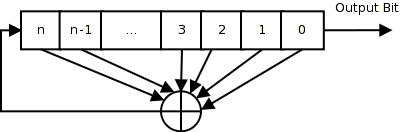
\includegraphics[scale=0.5]{lfsr}
    \caption{Linear feedback shift register (Fibonacci configuration)}
    \label{fig:lfsr-fib}
\end{figure}
Another type of LFSR is called a Galois configuration. It has the same
properties, but the feedback scheme is different: each bit in the tap sequence
is XORed with the output bit and replaced; the output bit then becomes the new
left-most bit (see Figure \ref{fig:lfsr-galois}).
\begin{figure}[htbp]
    \centering
    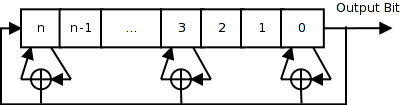
\includegraphics[scale=0.5]{lfsr_galois}
    \caption{Linear feedback shift register (Galois configuration)}
    \label{fig:lfsr-galois}
\end{figure}
A sequence generated by LFSR is linear by itself and therefore useless for
cryptography. It is possible to recover the LFSR structure from intercepting
only $2n$ bits of the generator using Berlekamp-Massey algorithm~\cite{joux:algorithmic_cryptanalysis}. 

Feedback with carry shift registers (FCSR) are similar to LFSRs but instead of
XORing the tapping sequence bits are added to the carry register. The result
reduced modulo 2 becomes the feedback bit of the register and the result divided
by 2 becomes the new value of the carry register.

The carry register has to be at least $\log_2 t$, where $t$ is the number of
taps. Thus, before the carry register is
filled there are some states of FCSR that never repeat. The maximum period of
FCSR differs from the one of LFSR. It equals to $q - 1$, where $q$ is the
connection integer and defined as 
$q = 2 q_1 + 2^2 q_2 + 2^4 q_4 + \cdots + 2^n q_n - 1$; $q$ has to be a prime
for which 2 is a primitive root. In fact not every initial state guarantees
maximum period of the register. That means the all pseudo-random sequence
generators based on FCSR will have a set of weak
keys~\cite{schneier:applied_cryptography:2}.

Non-linear feedback shift registers (NLFSR) use non-linear feedback function.
Such stream ciphers as Grain and Trivium are based on NLFSRs.  The idea both
behind NLFSRs and FCSRs is to ensure high non-linearity of the output sequence.
However such non-linear behavior makes the analysis of these registers almost
impossible. The described registers are unpredictable --- they don't guarantee
the maximal-period sequence, which also depends on the register initial state,
output sequences may have biases of zeroes and ones or contain long bit series.
Hereby, the advantage of these registers may at the same time lead to critical
flaw. Consequently, NLFSRs and FCSRs should be used with utmost caution.


\subsubsection{Clock control}

Clock control is one of several ways to introduce high nonlinearity in
pseudo-random sequence generated by linear feedback shift registers. The rate of
registers clocking varies either depending on several LFSRs or on certain bits
of the register state~\cite{usm:streamciphers}. As will be shown further, the combination of clock
control, combination and filter generators allow to form a pseudo-random
sequence satisfying all statistic requirements and yet resistant to known
attacks.

\subsubsection{Generators}                          

The use of feedback shift registers for cryptographic applications is possible by
combining several registers into a single generator. 

\subsubsection{Combination generators} 
The technique of combining outputs of several
registers by a Boolean function is called combination generator (see
Figure~\ref{fig:comb-gen}). The output sequence $s_t$ of a combination generator
composed on $n$ LFSRs is given by
\begin{equation}
    \label{eqn:comb-gen-seq}
    s_t = f(u_1, u_2, \cdots, u_n), \enspace \forall t \leq 0 \enspace, 
\end{equation}
where $u_i$ denotes the sequence generated by the $i$-th LFSR and $f$ is a
function of $n$ variables~\cite{encyclopedia_of_cryptography}.
\begin{figure}[htbp]
    \centering
    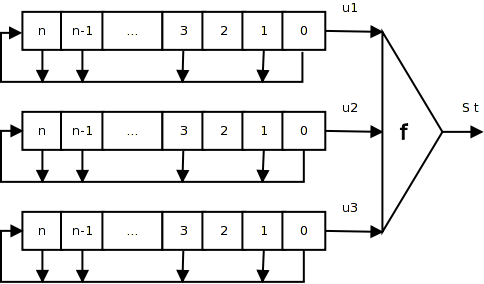
\includegraphics[scale=0.5]{comb-gen}
    \caption{Combination generator}
    \label{fig:comb-gen}
\end{figure}
The output of the $f$ function must be uniformly distributed and balanced in
order to produce pseudo-random sequences.

Linear complexity of the keystream generated by a combination generator composed
of $n$ LFSRs with primitive feedback polynomials combined by a Boolean function
$f$ equals to 
\begin{equation}
    \label{eqn:lin-complexity}
    f(L_1, L_2, \cdots, L_n) \enspace, 
\end{equation}
where the algebraic normal form of $f$ is evaluated over
integers and all lengths $L_1, \cdots, L_n$ are distinct and greater than 2.
High linear complexity of the generator is required to ensure that
Berlekamp-Massey algorithm is computationally infeasible.

Combination generators are vulnerable to correlation attacks which a based on 
recovering the initial states of all LFSRs from the knowledge of some sequence
produced by the generator (known plaintext attack). In order to protect
generators from this kind of attacks, the LFSR feedback polynomials should not
be sparse to ensure a high correlation-immunity order of a combining function.
However the correlation-immunity of a balanced Boolean function of $n$ variables
is limited with $n - 1 - deg(f)$~\cite{encyclopedia_of_cryptography}. Tradeoffs
between high algebraic degree,  high nonlinearity and high correlation-immunity
may be outwitted by replacing the combining function by a finite state automaton
with memory.

\subsubsection{Filter generators}
Filter generators, in distinction of combination generators, consist of a single
LFSR and its state is filtered by a nonlinear function~(see Figure
\ref{fig:filter-gen}). The output of the function is the pseudo-random sequence
formed by the generator. Just like in combination generators the filtering
function must be uniformly distributed and balanced.
\begin{figure}[htbp]
    \centering
    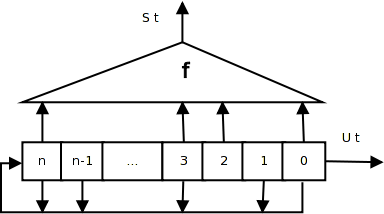
\includegraphics[scale=0.5]{filter-gen}
    \caption{Filter generator}
    \label{fig:filter-gen}
\end{figure}

Any filter generator can be represented by a corresponding combination generator
consisting of $n$ copies of the LFSR with shifted initial states when the
combining function complies the filtering function.

Filter generators are vulnerable to fast correlation and generalized inversion
attacks. Filtering function should be highly nonlinear in order to resist the
fast correlation attack. The inversion attack depends on the largest spacing
between two taps of the LFSR which conflicts with the statement that LFSRs
should use dense polynomials. Also the greatest common divisor of all spaces
between taps should equal to 1 or else the inversion attack could be
simplified~\cite{encyclopedia_of_cryptography}. 

Algebraic attacks are also applicable to filter generators since a keystream
bit can be represented by a function of $L$ initial bits of the LFSR. Therefore,
knowing $N$ keystream bits allows to form an algebraic system of $N$ equations
of $L$ variables. Using Gr\"obner bases (which may be viewed as nonlinear
generalization of Gaussian elimination for linear systems) enable an attacker to
lower the degree of the equations until the recovery of LFSR initial state is
possible by solving the algebraic system even with a filtering function of high
degree. 

Some of LFSR-based generators designs that promise to be secure are considered
further.

\subsubsection{Alternating stop-and-go generator}

The generator uses three LFSRs of different length. LFSR-1 controls clocking of
the other two. If output of LFSR-1 is 0, LFSR-3 is clocked, if its output is 1,
LFSR-2 is clocked. The output of the generator is the XOR of LFSR-2 and LFSR-3.
A correlation attack on LFSR-1 exists, but it does not threaten the generator
security~\cite{schneier:applied_cryptography:2}.

\subsubsection{Bilateral stop-and-go generator}

This generator uses two LFSRs of length $n$ and the output of the generator is
XOR of the outputs of each LFSR. The functioning of the generator is described
by algorithm~\ref{alg:stop-go-gen}.

\begin{algorithm}
    \caption{Bilateral stop-and-go generator functioning}
    \label{alg:stop-go-gen}
    \SetKw{Land}{and}
    \SetKwData{LfsrI}{LFSR-1}
    \SetKwData{LfsrII}{LFSR-2}
    \SetKwFunction{Output}{Output of}
    \SetKwFunction{Block}{Block}
    % It's \DontPrintSemicolon since release 4.0
    \dontprintsemicolon

    \If{\Output{\LfsrII at time $t-1$} == $0$ \Land \; 
    \Indp \Output{\LfsrII at time $t-2$} == $1$ \;}{
    \Block(\LfsrII at time $t$)
    }\;
    \If{\Output{\LfsrI at time $t-1$} == $0$ \Land \; 
    \Indp \Output{\LfsrI at time $t-2$} == $1$ \Land \;
    \LfsrI clocked at time $t$ \;}{
    \Block(\LfsrII at time $t$)
    }\;
\end{algorithm}

So far no critical attacks on this generator have been presented.

Another alternative is called filter generator and consists in
forming cryptographically strong pseudo-random sequence as some nonlinear
function of the state of a single register~\cite{robshaw:rsa:streamciphers}.

\subsubsection{Shrinking generator}

The idea behind shrinking generator is simple and uses two LFSRs. Both of them
are clocked each time: if the output of LFSR-1 is 1, then the generator output
is a bit from LFSR-2, otherwise both bits are discarded and the LFSRs are
clocked again.

The generator is said to be secure if no sparse polynomials are used in LFSRs,
but the downside is the irregular output rate. This problem can be solved by
buffering though it complicates implementation. 

\subsubsection{Self-shrinking generator}

The idea is similar to shrinking generator but uses pairs of bits from a single
LFSR. After clocking the register twice output bits are analysed: if the first
bit is 1, the output is the second bit; if the first bit is 0, bits are
discarded and the register is clocked again.

This generator is slower but requires less memory. However its properties are
unexplainable and hard to analyse.

\subsubsection{T-functions}

A new building block for symmetric ciphers called T-function was introduced by
Klimov and Shamir in 2003. T-function is a class of invertible mappings that
mixes arithmetic and boolean operations and processes full machine
words~\cite{klimov:tfunc}. 

Consider a construction where each input variable has $n$ bits, and $m$ input
variables are placed in the $m$ rows of an $m \times n$ bit matrix. Than a
T-function is defined by mapping
\begin{equation}
    \label{eqn:t-func}
    f: \mathbb{B}^{m \times n} \rightarrow \mathbb{B}^{k \times n} \enspace,
\end{equation}%
where $\mathbb{B} = \{0, 1\}$ and each $k$-th column of the output depends only on
the first $k$ columns of the input. In general, in order to compute the $k$-th
output bit only input bits $0, 1, \cdots, k$ must be known. Most machine
instructions are T-functions: negation, addition, subtraction, multiplication, left
shift (which is identical to multiplication by 2). Any combination of
T-functions is also a T-function.

The name of such transformation refers to the triangular dependence of the following
form~\cite{dblp:conf/fse/klimovs05}:
\begin{equation}
    \left(
    \begin{array}{c}
        \left[ f(x) \right]_0 \\
        \left[ f(x) \right]_1 \\
        \left[ f(x) \right]_2 \\
        \vdots \\
        \left[ f(x) \right]_{n-1} \\
    \end{array} \right)%
    = \left(
    \begin{array}{c}
        f_0([x]_0) \\
        f_1([x]_0, [x]_1) \\
        f_2([x]_0, [x]_1, [x]_2) \\
        \vdots \\
        f_{n-1}([x]_0, \cdots, [x]_{n-2}, [x]_{n-1})
    \end{array} \right) \enspace, 
\end{equation}
where $\left[ f(x) \right]_k$ is the $k$-th output column and 
$[x]k-1, \cdots, [x]_0$ --- first $k$ input columns.

The primary advantage of T-functions is computation efficiency both in hardware
and software implementation on modern processors. In spite of having desirable
cryptographic properties, some functions revealed weaknesses to correlation
attacks, distinguishing attacks~\cite{mycrypt/kunzli_jm05} with a complexity of
$2^{32}$ and algebraic attacks. Even though the use of T-functions is highly
attractive, reasonable security of such transformations should be proved.

\subsection{Well known ciphers}

Stream ciphers are essential for securing data in mobile communication systems.
This section reviews some latest stream ciphers designs considered for usage in
GSM, LTE and UMTS standards.

\subsubsection{A5/1}

A5/1 is a synchronous stream cipher based on three LFSRs of lengths 19, 22 and
23. The corresponding characteristic polynomials are sparse: 
\begin{equation}
    \begin{array}{ll}
        x^{19} + x^5 + x^2 + x + 1 \enspace, \\ 
        x^{22} + x + 1 \enspace, \\
        x^{23} + x^{15} + x^2 + x + 1 \enspace. 
    \end{array}
\end{equation}
The initial state of the generator depends on a 64-bit key $K$ and on a 22-bit
public frame number $F$. All three registers are zeroed, then clocked at time
$t = 1, \cdots, 64$ and the key bit $K_t$ is XORed to the feedback bit of each
LFSR. After the secret key is used, the feedback bit is XORed with $(t-64)$-th
it of the frame number. This initialization runs for 86 cycles.

Each LFSR has a clocking tap: tap 8 for LFSR-1, tap 10 for LFSR-2 and LFSR-3.
Then the majority $b$ of 3 clocking bits is computed and a certain LFSR is
clocked only if its clocking bit is equal to $b$. The generator output is
a XOR of outputs of all three LFSRs. After generating 328 bits of pseudo-random
sequence the first 100 ones are discarded and the rest (227 bits) form the
keystream.

A5/1 cipher can be broken within seconds using a combined distributed
rainbow table code book to decrypt GSM voice calls and text
messages~\cite{secproject}. 
The weakness of A5/1 stream
cipher originates from short feedback shift registers that use sparse
polynomials though it is efficient and has good statistical characteristics.

\subsubsection{Snow 3G}

Adoption and deployment of new cryptographic algorithms in global systems takes
a long time. Therefore the 3rd Generation Partnership Project (3GPP) decided to
develop promissory cipher suite in case the need of
transition~\cite{3gpp:uea2_doc1}. Despite the absence of evident weaknesses in
current KASUMI-based algorithms, new ciphers should be fundamentally distinct.
Thereby new attacks on existing cryptographic schemes will not be applicable to
the newly developed algorithms.

Over the time 3GPP has developed some requirements for cryptographic
confidentiality algorithms~\cite{3gpp:uea2_doc5}:
\begin{itemize}
    \item the algorithm shall only be used to protect the confidentiality of user
        data and signalling data sent over the radio access link between user
        equipment and radio network controller; the data is
        transmitted in plaintext once it reaches radio base station;
    \item the algorithm should be designed to accommodate a range of implementation
        options including hardware and software implementations; this
        requirement will make the deployment in telecommunication systems faster
        and more effective;
    \item for hardware implementations, it should be possible to implement one
        instance of the algorithm using less than $10000$ gates (working
        assumption); this ensures the possibility of algorithm implementation on
        various devices;
    \item it must be possible to implement the algorithm to achieve an encryption
        speed in the order of 10~Mbit/s on the downlink and on the uplink; this
        throughput should be available at a minimal clock speed of 
        \mbox{$20 \, \text{MHz}$};  
    \item the algorithm will be used to encrypt frames
            of variable length up to approximately 20000 bits;
    \item the algorithm should be a symmetric synchronous stream cipher;
    \item the length of the cipher key $CK$ is 128 bits; in case the effective key
        length should need to be made smaller than 128 bits, the most significant
        bits of $CK$ shall carry the effective key information, whereas the remaining,
        least significant bits shall be set zero;
    \item additional input parameters: COUNT, BEARER and DIRECTION compose the
        initialization vector (IV);
    \item plaintext block to be encrypted in a single $10$~ms physical layer frame
        for a given bearer and transmission direction.
\end{itemize}

In order to satisfy the described requirements, UMTS Encryption and Integrity
Algorithms (UEA2 and UIA2) were based on SNOW~3G stream
cipher~\cite{3gpp:uea2_doc2}.

SNOW is word-based synchronous stream cipher developed by Thomas Johansson
and Patrick Ekdahl. It was later modified to satisfy 3GPP Security Group
requirements and named SNOW~3G.

The structure of SNOW~3G is illustrated on figure~\ref{fig:snow3g_keystream}.
\begin{figure}[htbp]
    \centering
    % Graphic for TeX using PGF
% Title: /home/zoresvit/Dropbox/documents/research/diploma/graphics/snow3g_keystream.dia
% Creator: Dia v0.97.1
% CreationDate: Wed Nov  9 01:02:46 2011
% For: zoresvit
% \usepackage{tikz}
% The following commands are not supported in PSTricks at present
% We define them conditionally, so when they are implemented,
% this pgf file will use them.
\ifx\du\undefined
  \newlength{\du}
\fi
\setlength{\du}{12\unitlength}
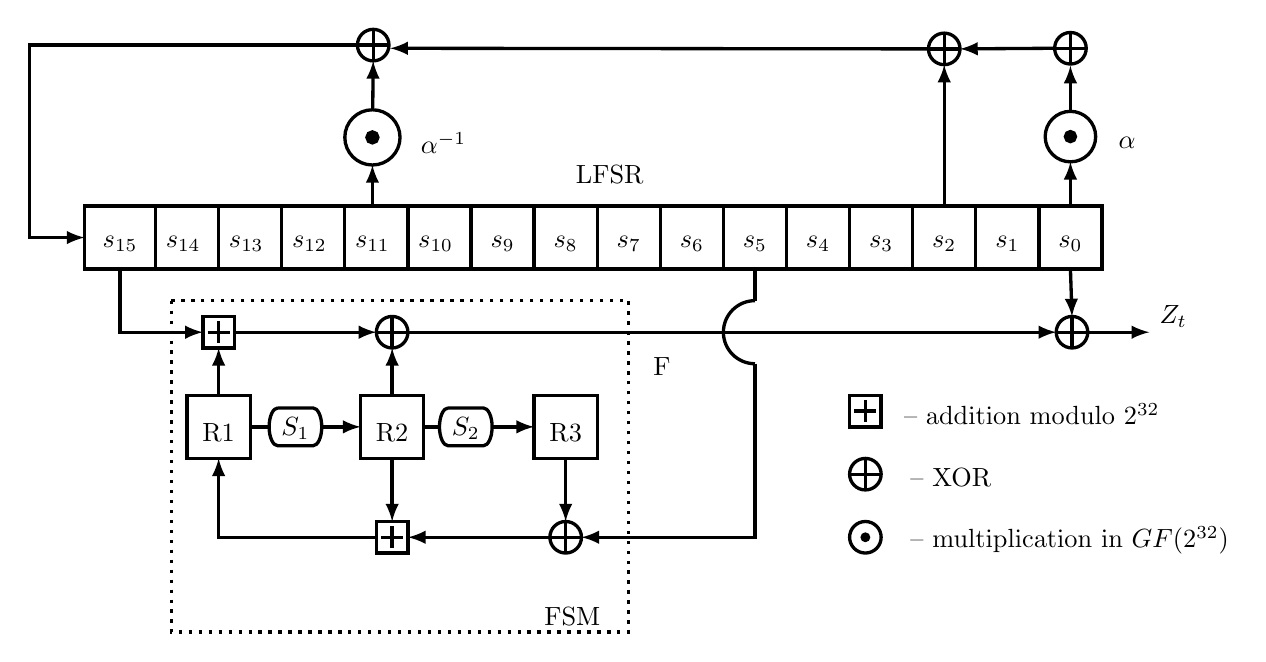
\begin{tikzpicture}[scale=0.95,every node/.style={scale=0.95}]
\pgftransformxscale{1.000000}
\pgftransformyscale{-1.000000}
\definecolor{dialinecolor}{rgb}{0.000000, 0.000000, 0.000000}
\pgfsetstrokecolor{dialinecolor}
\definecolor{dialinecolor}{rgb}{1.000000, 1.000000, 1.000000}
\pgfsetfillcolor{dialinecolor}
\definecolor{dialinecolor}{rgb}{1.000000, 1.000000, 1.000000}
\pgfsetfillcolor{dialinecolor}
\fill (40.000000\du,4.000000\du)--(40.000000\du,6.000000\du)--(42.000000\du,6.000000\du)--(42.000000\du,4.000000\du)--cycle;
\pgfsetlinewidth{0.100000\du}
\pgfsetdash{}{0pt}
\pgfsetdash{}{0pt}
\pgfsetmiterjoin
\definecolor{dialinecolor}{rgb}{0.000000, 0.000000, 0.000000}
\pgfsetstrokecolor{dialinecolor}
\draw (40.000000\du,4.000000\du)--(40.000000\du,6.000000\du)--(42.000000\du,6.000000\du)--(42.000000\du,4.000000\du)--cycle;
% setfont left to latex
\definecolor{dialinecolor}{rgb}{0.000000, 0.000000, 0.000000}
\pgfsetstrokecolor{dialinecolor}
\node at (41.000000\du,5.195000\du){$s_{0}$};
\definecolor{dialinecolor}{rgb}{1.000000, 1.000000, 1.000000}
\pgfsetfillcolor{dialinecolor}
\fill (38.000000\du,4.000000\du)--(38.000000\du,6.000000\du)--(40.000000\du,6.000000\du)--(40.000000\du,4.000000\du)--cycle;
\pgfsetlinewidth{0.100000\du}
\pgfsetdash{}{0pt}
\pgfsetdash{}{0pt}
\pgfsetmiterjoin
\definecolor{dialinecolor}{rgb}{0.000000, 0.000000, 0.000000}
\pgfsetstrokecolor{dialinecolor}
\draw (38.000000\du,4.000000\du)--(38.000000\du,6.000000\du)--(40.000000\du,6.000000\du)--(40.000000\du,4.000000\du)--cycle;
% setfont left to latex
\definecolor{dialinecolor}{rgb}{0.000000, 0.000000, 0.000000}
\pgfsetstrokecolor{dialinecolor}
\node at (39.000000\du,5.195000\du){$s_{1}$};
\definecolor{dialinecolor}{rgb}{1.000000, 1.000000, 1.000000}
\pgfsetfillcolor{dialinecolor}
\fill (36.000000\du,4.000000\du)--(36.000000\du,6.000000\du)--(38.000000\du,6.000000\du)--(38.000000\du,4.000000\du)--cycle;
\pgfsetlinewidth{0.100000\du}
\pgfsetdash{}{0pt}
\pgfsetdash{}{0pt}
\pgfsetmiterjoin
\definecolor{dialinecolor}{rgb}{0.000000, 0.000000, 0.000000}
\pgfsetstrokecolor{dialinecolor}
\draw (36.000000\du,4.000000\du)--(36.000000\du,6.000000\du)--(38.000000\du,6.000000\du)--(38.000000\du,4.000000\du)--cycle;
% setfont left to latex
\definecolor{dialinecolor}{rgb}{0.000000, 0.000000, 0.000000}
\pgfsetstrokecolor{dialinecolor}
\node at (37.000000\du,5.195000\du){$s_{2}$};
\definecolor{dialinecolor}{rgb}{1.000000, 1.000000, 1.000000}
\pgfsetfillcolor{dialinecolor}
\fill (34.000000\du,4.000000\du)--(34.000000\du,6.000000\du)--(36.000000\du,6.000000\du)--(36.000000\du,4.000000\du)--cycle;
\pgfsetlinewidth{0.100000\du}
\pgfsetdash{}{0pt}
\pgfsetdash{}{0pt}
\pgfsetmiterjoin
\definecolor{dialinecolor}{rgb}{0.000000, 0.000000, 0.000000}
\pgfsetstrokecolor{dialinecolor}
\draw (34.000000\du,4.000000\du)--(34.000000\du,6.000000\du)--(36.000000\du,6.000000\du)--(36.000000\du,4.000000\du)--cycle;
% setfont left to latex
\definecolor{dialinecolor}{rgb}{0.000000, 0.000000, 0.000000}
\pgfsetstrokecolor{dialinecolor}
\node at (35.000000\du,5.195000\du){$s_{3}$};
\definecolor{dialinecolor}{rgb}{1.000000, 1.000000, 1.000000}
\pgfsetfillcolor{dialinecolor}
\fill (32.000000\du,4.000000\du)--(32.000000\du,6.000000\du)--(34.000000\du,6.000000\du)--(34.000000\du,4.000000\du)--cycle;
\pgfsetlinewidth{0.100000\du}
\pgfsetdash{}{0pt}
\pgfsetdash{}{0pt}
\pgfsetmiterjoin
\definecolor{dialinecolor}{rgb}{0.000000, 0.000000, 0.000000}
\pgfsetstrokecolor{dialinecolor}
\draw (32.000000\du,4.000000\du)--(32.000000\du,6.000000\du)--(34.000000\du,6.000000\du)--(34.000000\du,4.000000\du)--cycle;
% setfont left to latex
\definecolor{dialinecolor}{rgb}{0.000000, 0.000000, 0.000000}
\pgfsetstrokecolor{dialinecolor}
\node at (33.000000\du,5.195000\du){$s_{4}$};
\definecolor{dialinecolor}{rgb}{1.000000, 1.000000, 1.000000}
\pgfsetfillcolor{dialinecolor}
\fill (30.000000\du,4.000000\du)--(30.000000\du,6.000000\du)--(32.000000\du,6.000000\du)--(32.000000\du,4.000000\du)--cycle;
\pgfsetlinewidth{0.100000\du}
\pgfsetdash{}{0pt}
\pgfsetdash{}{0pt}
\pgfsetmiterjoin
\definecolor{dialinecolor}{rgb}{0.000000, 0.000000, 0.000000}
\pgfsetstrokecolor{dialinecolor}
\draw (30.000000\du,4.000000\du)--(30.000000\du,6.000000\du)--(32.000000\du,6.000000\du)--(32.000000\du,4.000000\du)--cycle;
% setfont left to latex
\definecolor{dialinecolor}{rgb}{0.000000, 0.000000, 0.000000}
\pgfsetstrokecolor{dialinecolor}
\node at (31.000000\du,5.195000\du){$s_{5}$};
\definecolor{dialinecolor}{rgb}{1.000000, 1.000000, 1.000000}
\pgfsetfillcolor{dialinecolor}
\fill (28.000000\du,4.000000\du)--(28.000000\du,6.000000\du)--(30.000000\du,6.000000\du)--(30.000000\du,4.000000\du)--cycle;
\pgfsetlinewidth{0.100000\du}
\pgfsetdash{}{0pt}
\pgfsetdash{}{0pt}
\pgfsetmiterjoin
\definecolor{dialinecolor}{rgb}{0.000000, 0.000000, 0.000000}
\pgfsetstrokecolor{dialinecolor}
\draw (28.000000\du,4.000000\du)--(28.000000\du,6.000000\du)--(30.000000\du,6.000000\du)--(30.000000\du,4.000000\du)--cycle;
% setfont left to latex
\definecolor{dialinecolor}{rgb}{0.000000, 0.000000, 0.000000}
\pgfsetstrokecolor{dialinecolor}
\node at (29.000000\du,5.195000\du){$s_{6}$};
\definecolor{dialinecolor}{rgb}{1.000000, 1.000000, 1.000000}
\pgfsetfillcolor{dialinecolor}
\fill (26.000000\du,4.000000\du)--(26.000000\du,6.000000\du)--(28.000000\du,6.000000\du)--(28.000000\du,4.000000\du)--cycle;
\pgfsetlinewidth{0.100000\du}
\pgfsetdash{}{0pt}
\pgfsetdash{}{0pt}
\pgfsetmiterjoin
\definecolor{dialinecolor}{rgb}{0.000000, 0.000000, 0.000000}
\pgfsetstrokecolor{dialinecolor}
\draw (26.000000\du,4.000000\du)--(26.000000\du,6.000000\du)--(28.000000\du,6.000000\du)--(28.000000\du,4.000000\du)--cycle;
% setfont left to latex
\definecolor{dialinecolor}{rgb}{0.000000, 0.000000, 0.000000}
\pgfsetstrokecolor{dialinecolor}
\node at (27.000000\du,5.195000\du){$s_{7}$};
\definecolor{dialinecolor}{rgb}{1.000000, 1.000000, 1.000000}
\pgfsetfillcolor{dialinecolor}
\fill (24.000000\du,4.000000\du)--(24.000000\du,6.000000\du)--(26.000000\du,6.000000\du)--(26.000000\du,4.000000\du)--cycle;
\pgfsetlinewidth{0.100000\du}
\pgfsetdash{}{0pt}
\pgfsetdash{}{0pt}
\pgfsetmiterjoin
\definecolor{dialinecolor}{rgb}{0.000000, 0.000000, 0.000000}
\pgfsetstrokecolor{dialinecolor}
\draw (24.000000\du,4.000000\du)--(24.000000\du,6.000000\du)--(26.000000\du,6.000000\du)--(26.000000\du,4.000000\du)--cycle;
% setfont left to latex
\definecolor{dialinecolor}{rgb}{0.000000, 0.000000, 0.000000}
\pgfsetstrokecolor{dialinecolor}
\node at (25.000000\du,5.195000\du){$s_{8}$};
\definecolor{dialinecolor}{rgb}{1.000000, 1.000000, 1.000000}
\pgfsetfillcolor{dialinecolor}
\fill (22.000000\du,4.000000\du)--(22.000000\du,6.000000\du)--(24.000000\du,6.000000\du)--(24.000000\du,4.000000\du)--cycle;
\pgfsetlinewidth{0.100000\du}
\pgfsetdash{}{0pt}
\pgfsetdash{}{0pt}
\pgfsetmiterjoin
\definecolor{dialinecolor}{rgb}{0.000000, 0.000000, 0.000000}
\pgfsetstrokecolor{dialinecolor}
\draw (22.000000\du,4.000000\du)--(22.000000\du,6.000000\du)--(24.000000\du,6.000000\du)--(24.000000\du,4.000000\du)--cycle;
% setfont left to latex
\definecolor{dialinecolor}{rgb}{0.000000, 0.000000, 0.000000}
\pgfsetstrokecolor{dialinecolor}
\node at (23.000000\du,5.195000\du){$s_{9}$};
\definecolor{dialinecolor}{rgb}{1.000000, 1.000000, 1.000000}
\pgfsetfillcolor{dialinecolor}
\fill (19.750000\du,4.000000\du)--(19.750000\du,6.000000\du)--(22.000000\du,6.000000\du)--(22.000000\du,4.000000\du)--cycle;
\pgfsetlinewidth{0.100000\du}
\pgfsetdash{}{0pt}
\pgfsetdash{}{0pt}
\pgfsetmiterjoin
\definecolor{dialinecolor}{rgb}{0.000000, 0.000000, 0.000000}
\pgfsetstrokecolor{dialinecolor}
\draw (19.750000\du,4.000000\du)--(19.750000\du,6.000000\du)--(22.000000\du,6.000000\du)--(22.000000\du,4.000000\du)--cycle;
% setfont left to latex
\definecolor{dialinecolor}{rgb}{0.000000, 0.000000, 0.000000}
\pgfsetstrokecolor{dialinecolor}
\node at (20.875000\du,5.195000\du){$s_{10}$};
\definecolor{dialinecolor}{rgb}{1.000000, 1.000000, 1.000000}
\pgfsetfillcolor{dialinecolor}
\fill (17.750000\du,4.000000\du)--(17.750000\du,6.000000\du)--(20.000000\du,6.000000\du)--(20.000000\du,4.000000\du)--cycle;
\pgfsetlinewidth{0.100000\du}
\pgfsetdash{}{0pt}
\pgfsetdash{}{0pt}
\pgfsetmiterjoin
\definecolor{dialinecolor}{rgb}{0.000000, 0.000000, 0.000000}
\pgfsetstrokecolor{dialinecolor}
\draw (17.750000\du,4.000000\du)--(17.750000\du,6.000000\du)--(20.000000\du,6.000000\du)--(20.000000\du,4.000000\du)--cycle;
% setfont left to latex
\definecolor{dialinecolor}{rgb}{0.000000, 0.000000, 0.000000}
\pgfsetstrokecolor{dialinecolor}
\node at (18.875000\du,5.195000\du){$s_{11}$};
\definecolor{dialinecolor}{rgb}{1.000000, 1.000000, 1.000000}
\pgfsetfillcolor{dialinecolor}
\fill (15.750000\du,4.000000\du)--(15.750000\du,6.000000\du)--(18.000000\du,6.000000\du)--(18.000000\du,4.000000\du)--cycle;
\pgfsetlinewidth{0.100000\du}
\pgfsetdash{}{0pt}
\pgfsetdash{}{0pt}
\pgfsetmiterjoin
\definecolor{dialinecolor}{rgb}{0.000000, 0.000000, 0.000000}
\pgfsetstrokecolor{dialinecolor}
\draw (15.750000\du,4.000000\du)--(15.750000\du,6.000000\du)--(18.000000\du,6.000000\du)--(18.000000\du,4.000000\du)--cycle;
% setfont left to latex
\definecolor{dialinecolor}{rgb}{0.000000, 0.000000, 0.000000}
\pgfsetstrokecolor{dialinecolor}
\node at (16.875000\du,5.195000\du){$s_{12}$};
\definecolor{dialinecolor}{rgb}{1.000000, 1.000000, 1.000000}
\pgfsetfillcolor{dialinecolor}
\fill (13.750000\du,4.000000\du)--(13.750000\du,6.000000\du)--(16.000000\du,6.000000\du)--(16.000000\du,4.000000\du)--cycle;
\pgfsetlinewidth{0.100000\du}
\pgfsetdash{}{0pt}
\pgfsetdash{}{0pt}
\pgfsetmiterjoin
\definecolor{dialinecolor}{rgb}{0.000000, 0.000000, 0.000000}
\pgfsetstrokecolor{dialinecolor}
\draw (13.750000\du,4.000000\du)--(13.750000\du,6.000000\du)--(16.000000\du,6.000000\du)--(16.000000\du,4.000000\du)--cycle;
% setfont left to latex
\definecolor{dialinecolor}{rgb}{0.000000, 0.000000, 0.000000}
\pgfsetstrokecolor{dialinecolor}
\node at (14.875000\du,5.195000\du){$s_{13}$};
\definecolor{dialinecolor}{rgb}{1.000000, 1.000000, 1.000000}
\pgfsetfillcolor{dialinecolor}
\fill (11.750000\du,4.000000\du)--(11.750000\du,6.000000\du)--(14.000000\du,6.000000\du)--(14.000000\du,4.000000\du)--cycle;
\pgfsetlinewidth{0.100000\du}
\pgfsetdash{}{0pt}
\pgfsetdash{}{0pt}
\pgfsetmiterjoin
\definecolor{dialinecolor}{rgb}{0.000000, 0.000000, 0.000000}
\pgfsetstrokecolor{dialinecolor}
\draw (11.750000\du,4.000000\du)--(11.750000\du,6.000000\du)--(14.000000\du,6.000000\du)--(14.000000\du,4.000000\du)--cycle;
% setfont left to latex
\definecolor{dialinecolor}{rgb}{0.000000, 0.000000, 0.000000}
\pgfsetstrokecolor{dialinecolor}
\node at (12.875000\du,5.195000\du){$s_{14}$};
\definecolor{dialinecolor}{rgb}{1.000000, 1.000000, 1.000000}
\pgfsetfillcolor{dialinecolor}
\fill (9.750000\du,4.000000\du)--(9.750000\du,6.000000\du)--(12.000000\du,6.000000\du)--(12.000000\du,4.000000\du)--cycle;
\pgfsetlinewidth{0.100000\du}
\pgfsetdash{}{0pt}
\pgfsetdash{}{0pt}
\pgfsetmiterjoin
\definecolor{dialinecolor}{rgb}{0.000000, 0.000000, 0.000000}
\pgfsetstrokecolor{dialinecolor}
\draw (9.750000\du,4.000000\du)--(9.750000\du,6.000000\du)--(12.000000\du,6.000000\du)--(12.000000\du,4.000000\du)--cycle;
% setfont left to latex
\definecolor{dialinecolor}{rgb}{0.000000, 0.000000, 0.000000}
\pgfsetstrokecolor{dialinecolor}
\node at (10.875000\du,5.195000\du){$s_{15}$};
\definecolor{dialinecolor}{rgb}{1.000000, 1.000000, 1.000000}
\pgfsetfillcolor{dialinecolor}
\fill (13.000000\du,10.000000\du)--(13.000000\du,12.000000\du)--(15.000000\du,12.000000\du)--(15.000000\du,10.000000\du)--cycle;
\pgfsetlinewidth{0.100000\du}
\pgfsetdash{}{0pt}
\pgfsetdash{}{0pt}
\pgfsetmiterjoin
\definecolor{dialinecolor}{rgb}{0.000000, 0.000000, 0.000000}
\pgfsetstrokecolor{dialinecolor}
\draw (13.000000\du,10.000000\du)--(13.000000\du,12.000000\du)--(15.000000\du,12.000000\du)--(15.000000\du,10.000000\du)--cycle;
% setfont left to latex
\definecolor{dialinecolor}{rgb}{0.000000, 0.000000, 0.000000}
\pgfsetstrokecolor{dialinecolor}
\node at (14.000000\du,11.195000\du){R1};
\definecolor{dialinecolor}{rgb}{1.000000, 1.000000, 1.000000}
\pgfsetfillcolor{dialinecolor}
\fill (18.500000\du,10.000000\du)--(18.500000\du,12.000000\du)--(20.500000\du,12.000000\du)--(20.500000\du,10.000000\du)--cycle;
\pgfsetlinewidth{0.100000\du}
\pgfsetdash{}{0pt}
\pgfsetdash{}{0pt}
\pgfsetmiterjoin
\definecolor{dialinecolor}{rgb}{0.000000, 0.000000, 0.000000}
\pgfsetstrokecolor{dialinecolor}
\draw (18.500000\du,10.000000\du)--(18.500000\du,12.000000\du)--(20.500000\du,12.000000\du)--(20.500000\du,10.000000\du)--cycle;
% setfont left to latex
\definecolor{dialinecolor}{rgb}{0.000000, 0.000000, 0.000000}
\pgfsetstrokecolor{dialinecolor}
\node at (19.500000\du,11.195000\du){R2};
\definecolor{dialinecolor}{rgb}{1.000000, 1.000000, 1.000000}
\pgfsetfillcolor{dialinecolor}
\fill (24.000000\du,10.000000\du)--(24.000000\du,12.000000\du)--(26.000000\du,12.000000\du)--(26.000000\du,10.000000\du)--cycle;
\pgfsetlinewidth{0.100000\du}
\pgfsetdash{}{0pt}
\pgfsetdash{}{0pt}
\pgfsetmiterjoin
\definecolor{dialinecolor}{rgb}{0.000000, 0.000000, 0.000000}
\pgfsetstrokecolor{dialinecolor}
\draw (24.000000\du,10.000000\du)--(24.000000\du,12.000000\du)--(26.000000\du,12.000000\du)--(26.000000\du,10.000000\du)--cycle;
% setfont left to latex
\definecolor{dialinecolor}{rgb}{0.000000, 0.000000, 0.000000}
\pgfsetstrokecolor{dialinecolor}
\node at (25.000000\du,11.195000\du){R3};
\pgfsetlinewidth{0.100000\du}
\pgfsetdash{}{0pt}
\pgfsetdash{}{0pt}
\pgfsetbuttcap
\pgfsetmiterjoin
\pgfsetlinewidth{0.100000\du}
\pgfsetbuttcap
\pgfsetmiterjoin
\pgfsetdash{}{0pt}
\definecolor{dialinecolor}{rgb}{1.000000, 1.000000, 1.000000}
\pgfsetfillcolor{dialinecolor}
\pgfpathellipse{\pgfpoint{41.000000\du}{1.800000\du}}{\pgfpoint{0.800000\du}{0\du}}{\pgfpoint{0\du}{0.800000\du}}
\pgfusepath{fill}
\definecolor{dialinecolor}{rgb}{0.000000, 0.000000, 0.000000}
\pgfsetstrokecolor{dialinecolor}
\pgfpathellipse{\pgfpoint{41.000000\du}{1.800000\du}}{\pgfpoint{0.800000\du}{0\du}}{\pgfpoint{0\du}{0.800000\du}}
\pgfusepath{stroke}
\pgfsetbuttcap
\pgfsetmiterjoin
\pgfsetdash{}{0pt}
\definecolor{dialinecolor}{rgb}{0.000000, 0.000000, 0.000000}
\pgfsetfillcolor{dialinecolor}
\pgfpathellipse{\pgfpoint{41.000000\du}{1.800000\du}}{\pgfpoint{0.160000\du}{0\du}}{\pgfpoint{0\du}{0.160000\du}}
\pgfusepath{fill}
\definecolor{dialinecolor}{rgb}{0.000000, 0.000000, 0.000000}
\pgfsetstrokecolor{dialinecolor}
\pgfpathellipse{\pgfpoint{41.000000\du}{1.800000\du}}{\pgfpoint{0.160000\du}{0\du}}{\pgfpoint{0\du}{0.160000\du}}
\pgfusepath{stroke}
\pgfsetlinewidth{0.100000\du}
\pgfsetdash{}{0pt}
\pgfsetdash{}{0pt}
\pgfsetbuttcap
\pgfsetmiterjoin
\pgfsetlinewidth{0.100000\du}
\pgfsetbuttcap
\pgfsetmiterjoin
\pgfsetdash{}{0pt}
\definecolor{dialinecolor}{rgb}{1.000000, 1.000000, 1.000000}
\pgfsetfillcolor{dialinecolor}
\pgfpathellipse{\pgfpoint{41.050000\du}{8.000000\du}}{\pgfpoint{0.500000\du}{0\du}}{\pgfpoint{0\du}{0.500000\du}}
\pgfusepath{fill}
\definecolor{dialinecolor}{rgb}{0.000000, 0.000000, 0.000000}
\pgfsetstrokecolor{dialinecolor}
\pgfpathellipse{\pgfpoint{41.050000\du}{8.000000\du}}{\pgfpoint{0.500000\du}{0\du}}{\pgfpoint{0\du}{0.500000\du}}
\pgfusepath{stroke}
\pgfsetbuttcap
\pgfsetmiterjoin
\pgfsetdash{}{0pt}
\definecolor{dialinecolor}{rgb}{0.000000, 0.000000, 0.000000}
\pgfsetstrokecolor{dialinecolor}
\draw (41.050000\du,7.500000\du)--(41.050000\du,8.500000\du);
\pgfsetbuttcap
\pgfsetmiterjoin
\pgfsetdash{}{0pt}
\definecolor{dialinecolor}{rgb}{0.000000, 0.000000, 0.000000}
\pgfsetstrokecolor{dialinecolor}
\draw (40.550000\du,8.000000\du)--(41.550000\du,8.000000\du);
\pgfsetlinewidth{0.100000\du}
\pgfsetdash{}{0pt}
\pgfsetdash{}{0pt}
\pgfsetbuttcap
\pgfsetmiterjoin
\pgfsetlinewidth{0.100000\du}
\pgfsetbuttcap
\pgfsetmiterjoin
\pgfsetdash{}{0pt}
\definecolor{dialinecolor}{rgb}{1.000000, 1.000000, 1.000000}
\pgfsetfillcolor{dialinecolor}
\pgfpathellipse{\pgfpoint{41.000000\du}{-1.000000\du}}{\pgfpoint{0.500000\du}{0\du}}{\pgfpoint{0\du}{0.500000\du}}
\pgfusepath{fill}
\definecolor{dialinecolor}{rgb}{0.000000, 0.000000, 0.000000}
\pgfsetstrokecolor{dialinecolor}
\pgfpathellipse{\pgfpoint{41.000000\du}{-1.000000\du}}{\pgfpoint{0.500000\du}{0\du}}{\pgfpoint{0\du}{0.500000\du}}
\pgfusepath{stroke}
\pgfsetbuttcap
\pgfsetmiterjoin
\pgfsetdash{}{0pt}
\definecolor{dialinecolor}{rgb}{0.000000, 0.000000, 0.000000}
\pgfsetstrokecolor{dialinecolor}
\draw (41.000000\du,-1.500000\du)--(41.000000\du,-0.500000\du);
\pgfsetbuttcap
\pgfsetmiterjoin
\pgfsetdash{}{0pt}
\definecolor{dialinecolor}{rgb}{0.000000, 0.000000, 0.000000}
\pgfsetstrokecolor{dialinecolor}
\draw (40.500000\du,-1.000000\du)--(41.500000\du,-1.000000\du);
\pgfsetlinewidth{0.100000\du}
\pgfsetdash{}{0pt}
\pgfsetdash{}{0pt}
\pgfsetbuttcap
\pgfsetmiterjoin
\pgfsetlinewidth{0.100000\du}
\pgfsetbuttcap
\pgfsetmiterjoin
\pgfsetdash{}{0pt}
\definecolor{dialinecolor}{rgb}{1.000000, 1.000000, 1.000000}
\pgfsetfillcolor{dialinecolor}
\pgfpathellipse{\pgfpoint{37.000000\du}{-0.980000\du}}{\pgfpoint{0.500000\du}{0\du}}{\pgfpoint{0\du}{0.500000\du}}
\pgfusepath{fill}
\definecolor{dialinecolor}{rgb}{0.000000, 0.000000, 0.000000}
\pgfsetstrokecolor{dialinecolor}
\pgfpathellipse{\pgfpoint{37.000000\du}{-0.980000\du}}{\pgfpoint{0.500000\du}{0\du}}{\pgfpoint{0\du}{0.500000\du}}
\pgfusepath{stroke}
\pgfsetbuttcap
\pgfsetmiterjoin
\pgfsetdash{}{0pt}
\definecolor{dialinecolor}{rgb}{0.000000, 0.000000, 0.000000}
\pgfsetstrokecolor{dialinecolor}
\draw (37.000000\du,-1.480000\du)--(37.000000\du,-0.480000\du);
\pgfsetbuttcap
\pgfsetmiterjoin
\pgfsetdash{}{0pt}
\definecolor{dialinecolor}{rgb}{0.000000, 0.000000, 0.000000}
\pgfsetstrokecolor{dialinecolor}
\draw (36.500000\du,-0.980000\du)--(37.500000\du,-0.980000\du);
\pgfsetlinewidth{0.100000\du}
\pgfsetdash{}{0pt}
\pgfsetdash{}{0pt}
\pgfsetbuttcap
\pgfsetmiterjoin
\pgfsetlinewidth{0.100000\du}
\pgfsetbuttcap
\pgfsetmiterjoin
\pgfsetdash{}{0pt}
\definecolor{dialinecolor}{rgb}{1.000000, 1.000000, 1.000000}
\pgfsetfillcolor{dialinecolor}
\pgfpathellipse{\pgfpoint{18.900000\du}{-1.100000\du}}{\pgfpoint{0.500000\du}{0\du}}{\pgfpoint{0\du}{0.500000\du}}
\pgfusepath{fill}
\definecolor{dialinecolor}{rgb}{0.000000, 0.000000, 0.000000}
\pgfsetstrokecolor{dialinecolor}
\pgfpathellipse{\pgfpoint{18.900000\du}{-1.100000\du}}{\pgfpoint{0.500000\du}{0\du}}{\pgfpoint{0\du}{0.500000\du}}
\pgfusepath{stroke}
\pgfsetbuttcap
\pgfsetmiterjoin
\pgfsetdash{}{0pt}
\definecolor{dialinecolor}{rgb}{0.000000, 0.000000, 0.000000}
\pgfsetstrokecolor{dialinecolor}
\draw (18.900000\du,-1.600000\du)--(18.900000\du,-0.600000\du);
\pgfsetbuttcap
\pgfsetmiterjoin
\pgfsetdash{}{0pt}
\definecolor{dialinecolor}{rgb}{0.000000, 0.000000, 0.000000}
\pgfsetstrokecolor{dialinecolor}
\draw (18.400000\du,-1.100000\du)--(19.400000\du,-1.100000\du);
\pgfsetlinewidth{0.100000\du}
\pgfsetdash{}{0pt}
\pgfsetdash{}{0pt}
\pgfsetbuttcap
\pgfsetmiterjoin
\pgfsetlinewidth{0.100000\du}
\pgfsetbuttcap
\pgfsetmiterjoin
\pgfsetdash{}{0pt}
\definecolor{dialinecolor}{rgb}{1.000000, 1.000000, 1.000000}
\pgfsetfillcolor{dialinecolor}
\fill (13.500000\du,7.500000\du)--(13.500000\du,8.500000\du)--(14.500000\du,8.500000\du)--(14.500000\du,7.500000\du)--cycle;
\definecolor{dialinecolor}{rgb}{0.000000, 0.000000, 0.000000}
\pgfsetstrokecolor{dialinecolor}
\draw (13.500000\du,7.500000\du)--(13.500000\du,8.500000\du)--(14.500000\du,8.500000\du)--(14.500000\du,7.500000\du)--cycle;
\pgfsetbuttcap
\pgfsetmiterjoin
\pgfsetdash{}{0pt}
\definecolor{dialinecolor}{rgb}{0.000000, 0.000000, 0.000000}
\pgfsetstrokecolor{dialinecolor}
\draw (14.000000\du,7.650000\du)--(14.000000\du,8.350000\du);
\pgfsetbuttcap
\pgfsetmiterjoin
\pgfsetdash{}{0pt}
\definecolor{dialinecolor}{rgb}{0.000000, 0.000000, 0.000000}
\pgfsetstrokecolor{dialinecolor}
\draw (13.650000\du,8.000000\du)--(14.350000\du,8.000000\du);
\pgfsetlinewidth{0.100000\du}
\pgfsetdash{}{0pt}
\pgfsetdash{}{0pt}
\pgfsetbuttcap
\pgfsetmiterjoin
\pgfsetlinewidth{0.100000\du}
\pgfsetbuttcap
\pgfsetmiterjoin
\pgfsetdash{}{0pt}
\definecolor{dialinecolor}{rgb}{1.000000, 1.000000, 1.000000}
\pgfsetfillcolor{dialinecolor}
\fill (19.000000\du,14.000000\du)--(19.000000\du,15.000000\du)--(20.000000\du,15.000000\du)--(20.000000\du,14.000000\du)--cycle;
\definecolor{dialinecolor}{rgb}{0.000000, 0.000000, 0.000000}
\pgfsetstrokecolor{dialinecolor}
\draw (19.000000\du,14.000000\du)--(19.000000\du,15.000000\du)--(20.000000\du,15.000000\du)--(20.000000\du,14.000000\du)--cycle;
\pgfsetbuttcap
\pgfsetmiterjoin
\pgfsetdash{}{0pt}
\definecolor{dialinecolor}{rgb}{0.000000, 0.000000, 0.000000}
\pgfsetstrokecolor{dialinecolor}
\draw (19.500000\du,14.150000\du)--(19.500000\du,14.850000\du);
\pgfsetbuttcap
\pgfsetmiterjoin
\pgfsetdash{}{0pt}
\definecolor{dialinecolor}{rgb}{0.000000, 0.000000, 0.000000}
\pgfsetstrokecolor{dialinecolor}
\draw (19.150000\du,14.500000\du)--(19.850000\du,14.500000\du);
\pgfsetlinewidth{0.100000\du}
\pgfsetdash{}{0pt}
\pgfsetdash{}{0pt}
\pgfsetbuttcap
\pgfsetmiterjoin
\pgfsetlinewidth{0.100000\du}
\pgfsetbuttcap
\pgfsetmiterjoin
\pgfsetdash{}{0pt}
\definecolor{dialinecolor}{rgb}{1.000000, 1.000000, 1.000000}
\pgfsetfillcolor{dialinecolor}
\pgfpathellipse{\pgfpoint{25.000000\du}{14.500000\du}}{\pgfpoint{0.500000\du}{0\du}}{\pgfpoint{0\du}{0.500000\du}}
\pgfusepath{fill}
\definecolor{dialinecolor}{rgb}{0.000000, 0.000000, 0.000000}
\pgfsetstrokecolor{dialinecolor}
\pgfpathellipse{\pgfpoint{25.000000\du}{14.500000\du}}{\pgfpoint{0.500000\du}{0\du}}{\pgfpoint{0\du}{0.500000\du}}
\pgfusepath{stroke}
\pgfsetbuttcap
\pgfsetmiterjoin
\pgfsetdash{}{0pt}
\definecolor{dialinecolor}{rgb}{0.000000, 0.000000, 0.000000}
\pgfsetstrokecolor{dialinecolor}
\draw (25.000000\du,14.000000\du)--(25.000000\du,15.000000\du);
\pgfsetbuttcap
\pgfsetmiterjoin
\pgfsetdash{}{0pt}
\definecolor{dialinecolor}{rgb}{0.000000, 0.000000, 0.000000}
\pgfsetstrokecolor{dialinecolor}
\draw (24.500000\du,14.500000\du)--(25.500000\du,14.500000\du);
\pgfsetlinewidth{0.100000\du}
\pgfsetdash{}{0pt}
\pgfsetdash{}{0pt}
\pgfsetbuttcap
\pgfsetmiterjoin
\pgfsetlinewidth{0.100000\du}
\pgfsetbuttcap
\pgfsetmiterjoin
\pgfsetdash{}{0pt}
\definecolor{dialinecolor}{rgb}{1.000000, 1.000000, 1.000000}
\pgfsetfillcolor{dialinecolor}
\pgfpathellipse{\pgfpoint{19.500000\du}{8.000000\du}}{\pgfpoint{0.500000\du}{0\du}}{\pgfpoint{0\du}{0.500000\du}}
\pgfusepath{fill}
\definecolor{dialinecolor}{rgb}{0.000000, 0.000000, 0.000000}
\pgfsetstrokecolor{dialinecolor}
\pgfpathellipse{\pgfpoint{19.500000\du}{8.000000\du}}{\pgfpoint{0.500000\du}{0\du}}{\pgfpoint{0\du}{0.500000\du}}
\pgfusepath{stroke}
\pgfsetbuttcap
\pgfsetmiterjoin
\pgfsetdash{}{0pt}
\definecolor{dialinecolor}{rgb}{0.000000, 0.000000, 0.000000}
\pgfsetstrokecolor{dialinecolor}
\draw (19.500000\du,7.500000\du)--(19.500000\du,8.500000\du);
\pgfsetbuttcap
\pgfsetmiterjoin
\pgfsetdash{}{0pt}
\definecolor{dialinecolor}{rgb}{0.000000, 0.000000, 0.000000}
\pgfsetstrokecolor{dialinecolor}
\draw (19.000000\du,8.000000\du)--(20.000000\du,8.000000\du);
\pgfsetlinewidth{0.100000\du}
\pgfsetdash{}{0pt}
\pgfsetdash{}{0pt}
\pgfsetbuttcap
{
\definecolor{dialinecolor}{rgb}{0.000000, 0.000000, 0.000000}
\pgfsetfillcolor{dialinecolor}
% was here!!!
\pgfsetarrowsend{latex}
\definecolor{dialinecolor}{rgb}{0.000000, 0.000000, 0.000000}
\pgfsetstrokecolor{dialinecolor}
\draw (14.500000\du,8.000000\du)--(19.000000\du,8.000000\du);
}
\pgfsetlinewidth{0.100000\du}
\pgfsetdash{}{0pt}
\pgfsetdash{}{0pt}
\pgfsetbuttcap
{
\definecolor{dialinecolor}{rgb}{0.000000, 0.000000, 0.000000}
\pgfsetfillcolor{dialinecolor}
% was here!!!
\pgfsetarrowsend{latex}
\definecolor{dialinecolor}{rgb}{0.000000, 0.000000, 0.000000}
\pgfsetstrokecolor{dialinecolor}
\draw (14.000000\du,9.949890\du)--(14.000000\du,8.500000\du);
}
\pgfsetlinewidth{0.100000\du}
\pgfsetdash{}{0pt}
\pgfsetdash{}{0pt}
\pgfsetbuttcap
{
\definecolor{dialinecolor}{rgb}{0.000000, 0.000000, 0.000000}
\pgfsetfillcolor{dialinecolor}
% was here!!!
\pgfsetarrowsend{latex}
\definecolor{dialinecolor}{rgb}{0.000000, 0.000000, 0.000000}
\pgfsetstrokecolor{dialinecolor}
\draw (15.000000\du,11.000000\du)--(18.500000\du,11.000000\du);
}
\pgfsetlinewidth{0.100000\du}
\pgfsetdash{}{0pt}
\pgfsetdash{}{0pt}
\pgfsetbuttcap
\pgfsetmiterjoin
\pgfsetlinewidth{0.100000\du}
\pgfsetbuttcap
\pgfsetmiterjoin
\pgfsetdash{}{0pt}
\definecolor{dialinecolor}{rgb}{1.000000, 1.000000, 1.000000}
\pgfsetfillcolor{dialinecolor}
\pgfpathmoveto{\pgfpoint{15.878125\du}{10.400000\du}}
\pgfpathlineto{\pgfpoint{16.990625\du}{10.400000\du}}
\pgfpathcurveto{\pgfpoint{17.144229\du}{10.400000\du}}{\pgfpoint{17.268750\du}{10.668629\du}}{\pgfpoint{17.268750\du}{11.000000\du}}
\pgfpathcurveto{\pgfpoint{17.268750\du}{11.331371\du}}{\pgfpoint{17.144229\du}{11.600000\du}}{\pgfpoint{16.990625\du}{11.600000\du}}
\pgfpathlineto{\pgfpoint{15.878125\du}{11.600000\du}}
\pgfpathcurveto{\pgfpoint{15.724521\du}{11.600000\du}}{\pgfpoint{15.600000\du}{11.331371\du}}{\pgfpoint{15.600000\du}{11.000000\du}}
\pgfpathcurveto{\pgfpoint{15.600000\du}{10.668629\du}}{\pgfpoint{15.724521\du}{10.400000\du}}{\pgfpoint{15.878125\du}{10.400000\du}}
\pgfusepath{fill}
\definecolor{dialinecolor}{rgb}{0.000000, 0.000000, 0.000000}
\pgfsetstrokecolor{dialinecolor}
\pgfpathmoveto{\pgfpoint{15.878125\du}{10.400000\du}}
\pgfpathlineto{\pgfpoint{16.990625\du}{10.400000\du}}
\pgfpathcurveto{\pgfpoint{17.144229\du}{10.400000\du}}{\pgfpoint{17.268750\du}{10.668629\du}}{\pgfpoint{17.268750\du}{11.000000\du}}
\pgfpathcurveto{\pgfpoint{17.268750\du}{11.331371\du}}{\pgfpoint{17.144229\du}{11.600000\du}}{\pgfpoint{16.990625\du}{11.600000\du}}
\pgfpathlineto{\pgfpoint{15.878125\du}{11.600000\du}}
\pgfpathcurveto{\pgfpoint{15.724521\du}{11.600000\du}}{\pgfpoint{15.600000\du}{11.331371\du}}{\pgfpoint{15.600000\du}{11.000000\du}}
\pgfpathcurveto{\pgfpoint{15.600000\du}{10.668629\du}}{\pgfpoint{15.724521\du}{10.400000\du}}{\pgfpoint{15.878125\du}{10.400000\du}}
\pgfusepath{stroke}
% setfont left to latex
\definecolor{dialinecolor}{rgb}{0.000000, 0.000000, 0.000000}
\pgfsetstrokecolor{dialinecolor}
\node at (16.434375\du,11.050000\du){$S_{1}$};
\pgfsetlinewidth{0.100000\du}
\pgfsetdash{}{0pt}
\pgfsetdash{}{0pt}
\pgfsetbuttcap
{
\definecolor{dialinecolor}{rgb}{0.000000, 0.000000, 0.000000}
\pgfsetfillcolor{dialinecolor}
% was here!!!
\pgfsetarrowsend{latex}
\definecolor{dialinecolor}{rgb}{0.000000, 0.000000, 0.000000}
\pgfsetstrokecolor{dialinecolor}
\draw (20.500000\du,11.000000\du)--(24.000000\du,11.000000\du);
}
\pgfsetlinewidth{0.100000\du}
\pgfsetdash{}{0pt}
\pgfsetdash{}{0pt}
\pgfsetbuttcap
\pgfsetmiterjoin
\pgfsetlinewidth{0.100000\du}
\pgfsetbuttcap
\pgfsetmiterjoin
\pgfsetdash{}{0pt}
\definecolor{dialinecolor}{rgb}{1.000000, 1.000000, 1.000000}
\pgfsetfillcolor{dialinecolor}
\pgfpathmoveto{\pgfpoint{21.278125\du}{10.400000\du}}
\pgfpathlineto{\pgfpoint{22.390625\du}{10.400000\du}}
\pgfpathcurveto{\pgfpoint{22.544229\du}{10.400000\du}}{\pgfpoint{22.668750\du}{10.668629\du}}{\pgfpoint{22.668750\du}{11.000000\du}}
\pgfpathcurveto{\pgfpoint{22.668750\du}{11.331371\du}}{\pgfpoint{22.544229\du}{11.600000\du}}{\pgfpoint{22.390625\du}{11.600000\du}}
\pgfpathlineto{\pgfpoint{21.278125\du}{11.600000\du}}
\pgfpathcurveto{\pgfpoint{21.124521\du}{11.600000\du}}{\pgfpoint{21.000000\du}{11.331371\du}}{\pgfpoint{21.000000\du}{11.000000\du}}
\pgfpathcurveto{\pgfpoint{21.000000\du}{10.668629\du}}{\pgfpoint{21.124521\du}{10.400000\du}}{\pgfpoint{21.278125\du}{10.400000\du}}
\pgfusepath{fill}
\definecolor{dialinecolor}{rgb}{0.000000, 0.000000, 0.000000}
\pgfsetstrokecolor{dialinecolor}
\pgfpathmoveto{\pgfpoint{21.278125\du}{10.400000\du}}
\pgfpathlineto{\pgfpoint{22.390625\du}{10.400000\du}}
\pgfpathcurveto{\pgfpoint{22.544229\du}{10.400000\du}}{\pgfpoint{22.668750\du}{10.668629\du}}{\pgfpoint{22.668750\du}{11.000000\du}}
\pgfpathcurveto{\pgfpoint{22.668750\du}{11.331371\du}}{\pgfpoint{22.544229\du}{11.600000\du}}{\pgfpoint{22.390625\du}{11.600000\du}}
\pgfpathlineto{\pgfpoint{21.278125\du}{11.600000\du}}
\pgfpathcurveto{\pgfpoint{21.124521\du}{11.600000\du}}{\pgfpoint{21.000000\du}{11.331371\du}}{\pgfpoint{21.000000\du}{11.000000\du}}
\pgfpathcurveto{\pgfpoint{21.000000\du}{10.668629\du}}{\pgfpoint{21.124521\du}{10.400000\du}}{\pgfpoint{21.278125\du}{10.400000\du}}
\pgfusepath{stroke}
% setfont left to latex
\definecolor{dialinecolor}{rgb}{0.000000, 0.000000, 0.000000}
\pgfsetstrokecolor{dialinecolor}
\node at (21.834375\du,11.050000\du){$S_{2}$};
\pgfsetlinewidth{0.100000\du}
\pgfsetdash{}{0pt}
\pgfsetdash{}{0pt}
\pgfsetbuttcap
{
\definecolor{dialinecolor}{rgb}{0.000000, 0.000000, 0.000000}
\pgfsetfillcolor{dialinecolor}
% was here!!!
\pgfsetarrowsend{latex}
\definecolor{dialinecolor}{rgb}{0.000000, 0.000000, 0.000000}
\pgfsetstrokecolor{dialinecolor}
\draw (19.500000\du,12.000000\du)--(19.500000\du,14.000000\du);
}
\pgfsetlinewidth{0.100000\du}
\pgfsetdash{}{0pt}
\pgfsetdash{}{0pt}
\pgfsetbuttcap
{
\definecolor{dialinecolor}{rgb}{0.000000, 0.000000, 0.000000}
\pgfsetfillcolor{dialinecolor}
% was here!!!
\pgfsetarrowsend{latex}
\definecolor{dialinecolor}{rgb}{0.000000, 0.000000, 0.000000}
\pgfsetstrokecolor{dialinecolor}
\draw (25.000000\du,12.000000\du)--(25.000000\du,14.000000\du);
}
\pgfsetlinewidth{0.100000\du}
\pgfsetdash{}{0pt}
\pgfsetdash{}{0pt}
\pgfsetbuttcap
{
\definecolor{dialinecolor}{rgb}{0.000000, 0.000000, 0.000000}
\pgfsetfillcolor{dialinecolor}
% was here!!!
\pgfsetarrowsend{latex}
\definecolor{dialinecolor}{rgb}{0.000000, 0.000000, 0.000000}
\pgfsetstrokecolor{dialinecolor}
\draw (24.500000\du,14.500000\du)--(20.000000\du,14.500000\du);
}
\pgfsetlinewidth{0.100000\du}
\pgfsetdash{}{0pt}
\pgfsetdash{}{0pt}
\pgfsetmiterjoin
\pgfsetbuttcap
{
\definecolor{dialinecolor}{rgb}{0.000000, 0.000000, 0.000000}
\pgfsetfillcolor{dialinecolor}
% was here!!!
\pgfsetarrowsend{latex}
{\pgfsetcornersarced{\pgfpoint{0.000000\du}{0.000000\du}}\definecolor{dialinecolor}{rgb}{0.000000, 0.000000, 0.000000}
\pgfsetstrokecolor{dialinecolor}
\draw (19.000000\du,14.500000\du)--(14.000000\du,14.500000\du)--(14.000000\du,12.000000\du);
}}
\pgfsetlinewidth{0.100000\du}
\pgfsetdash{}{0pt}
\pgfsetdash{}{0pt}
\pgfsetbuttcap
{
\definecolor{dialinecolor}{rgb}{0.000000, 0.000000, 0.000000}
\pgfsetfillcolor{dialinecolor}
% was here!!!
\pgfsetarrowsend{latex}
\definecolor{dialinecolor}{rgb}{0.000000, 0.000000, 0.000000}
\pgfsetstrokecolor{dialinecolor}
\draw (19.500000\du,9.949890\du)--(19.500000\du,8.500000\du);
}
\pgfsetlinewidth{0.100000\du}
\pgfsetdash{}{0pt}
\pgfsetdash{}{0pt}
\pgfsetbuttcap
{
\definecolor{dialinecolor}{rgb}{0.000000, 0.000000, 0.000000}
\pgfsetfillcolor{dialinecolor}
% was here!!!
\pgfsetarrowsend{latex}
\definecolor{dialinecolor}{rgb}{0.000000, 0.000000, 0.000000}
\pgfsetstrokecolor{dialinecolor}
\draw (20.000000\du,8.000000\du)--(40.550000\du,8.000000\du);
}
\pgfsetlinewidth{0.100000\du}
\pgfsetdash{}{0pt}
\pgfsetdash{}{0pt}
\pgfsetbuttcap
{
\definecolor{dialinecolor}{rgb}{0.000000, 0.000000, 0.000000}
\pgfsetfillcolor{dialinecolor}
% was here!!!
\pgfsetarrowsend{latex}
\definecolor{dialinecolor}{rgb}{0.000000, 0.000000, 0.000000}
\pgfsetstrokecolor{dialinecolor}
\draw (41.000000\du,6.000000\du)--(41.050000\du,7.500000\du);
}
\pgfsetlinewidth{0.100000\du}
\pgfsetdash{}{0pt}
\pgfsetdash{}{0pt}
\pgfsetbuttcap
{
\definecolor{dialinecolor}{rgb}{0.000000, 0.000000, 0.000000}
\pgfsetfillcolor{dialinecolor}
% was here!!!
\pgfsetarrowsend{latex}
\definecolor{dialinecolor}{rgb}{0.000000, 0.000000, 0.000000}
\pgfsetstrokecolor{dialinecolor}
\draw (41.550000\du,8.000000\du)--(43.500000\du,8.000000\du);
}
% setfont left to latex
\definecolor{dialinecolor}{rgb}{0.000000, 0.000000, 0.000000}
\pgfsetstrokecolor{dialinecolor}
\node[anchor=west] at (43.500000\du,7.500000\du){$Z_t$};
\pgfsetlinewidth{0.100000\du}
\pgfsetdash{}{0pt}
\pgfsetdash{}{0pt}
\pgfsetbuttcap
{
\definecolor{dialinecolor}{rgb}{0.000000, 0.000000, 0.000000}
\pgfsetfillcolor{dialinecolor}
% was here!!!
\pgfsetarrowsend{latex}
\definecolor{dialinecolor}{rgb}{0.000000, 0.000000, 0.000000}
\pgfsetstrokecolor{dialinecolor}
\draw (41.000000\du,4.000000\du)--(41.000000\du,2.600000\du);
}
\pgfsetlinewidth{0.100000\du}
\pgfsetdash{}{0pt}
\pgfsetdash{}{0pt}
\pgfsetbuttcap
\pgfsetmiterjoin
\pgfsetlinewidth{0.100000\du}
\pgfsetbuttcap
\pgfsetmiterjoin
\pgfsetdash{}{0pt}
\definecolor{dialinecolor}{rgb}{1.000000, 1.000000, 1.000000}
\pgfsetfillcolor{dialinecolor}
\pgfpathellipse{\pgfpoint{18.875000\du}{1.825000\du}}{\pgfpoint{0.875000\du}{0\du}}{\pgfpoint{0\du}{0.875000\du}}
\pgfusepath{fill}
\definecolor{dialinecolor}{rgb}{0.000000, 0.000000, 0.000000}
\pgfsetstrokecolor{dialinecolor}
\pgfpathellipse{\pgfpoint{18.875000\du}{1.825000\du}}{\pgfpoint{0.875000\du}{0\du}}{\pgfpoint{0\du}{0.875000\du}}
\pgfusepath{stroke}
\pgfsetbuttcap
\pgfsetmiterjoin
\pgfsetdash{}{0pt}
\definecolor{dialinecolor}{rgb}{0.000000, 0.000000, 0.000000}
\pgfsetfillcolor{dialinecolor}
\pgfpathellipse{\pgfpoint{18.875000\du}{1.825000\du}}{\pgfpoint{0.175000\du}{0\du}}{\pgfpoint{0\du}{0.175000\du}}
\pgfusepath{fill}
\definecolor{dialinecolor}{rgb}{0.000000, 0.000000, 0.000000}
\pgfsetstrokecolor{dialinecolor}
\pgfpathellipse{\pgfpoint{18.875000\du}{1.825000\du}}{\pgfpoint{0.175000\du}{0\du}}{\pgfpoint{0\du}{0.175000\du}}
\pgfusepath{stroke}
\pgfsetlinewidth{0.100000\du}
\pgfsetdash{}{0pt}
\pgfsetdash{}{0pt}
\pgfsetbuttcap
{
\definecolor{dialinecolor}{rgb}{0.000000, 0.000000, 0.000000}
\pgfsetfillcolor{dialinecolor}
% was here!!!
\pgfsetarrowsend{latex}
\definecolor{dialinecolor}{rgb}{0.000000, 0.000000, 0.000000}
\pgfsetstrokecolor{dialinecolor}
\draw (41.000000\du,1.000000\du)--(41.000000\du,-0.450049\du);
}
\pgfsetlinewidth{0.100000\du}
\pgfsetdash{}{0pt}
\pgfsetdash{}{0pt}
\pgfsetbuttcap
{
\definecolor{dialinecolor}{rgb}{0.000000, 0.000000, 0.000000}
\pgfsetfillcolor{dialinecolor}
% was here!!!
\pgfsetarrowsend{latex}
\definecolor{dialinecolor}{rgb}{0.000000, 0.000000, 0.000000}
\pgfsetstrokecolor{dialinecolor}
\draw (40.500000\du,-1.000000\du)--(37.500000\du,-0.980000\du);
}
\pgfsetlinewidth{0.100000\du}
\pgfsetdash{}{0pt}
\pgfsetdash{}{0pt}
\pgfsetbuttcap
{
\definecolor{dialinecolor}{rgb}{0.000000, 0.000000, 0.000000}
\pgfsetfillcolor{dialinecolor}
% was here!!!
\pgfsetarrowsend{latex}
\definecolor{dialinecolor}{rgb}{0.000000, 0.000000, 0.000000}
\pgfsetstrokecolor{dialinecolor}
\draw (37.000000\du,4.000000\du)--(37.000000\du,-0.480000\du);
}
\pgfsetlinewidth{0.100000\du}
\pgfsetdash{}{0pt}
\pgfsetdash{}{0pt}
\pgfsetbuttcap
{
\definecolor{dialinecolor}{rgb}{0.000000, 0.000000, 0.000000}
\pgfsetfillcolor{dialinecolor}
% was here!!!
\pgfsetarrowsend{latex}
\definecolor{dialinecolor}{rgb}{0.000000, 0.000000, 0.000000}
\pgfsetstrokecolor{dialinecolor}
\draw (36.500000\du,-0.980000\du)--(19.437109\du,-0.999390\du);
}
\pgfsetlinewidth{0.100000\du}
\pgfsetdash{}{0pt}
\pgfsetdash{}{0pt}
\pgfsetbuttcap
{
\definecolor{dialinecolor}{rgb}{0.000000, 0.000000, 0.000000}
\pgfsetfillcolor{dialinecolor}
% was here!!!
\pgfsetarrowsend{latex}
\definecolor{dialinecolor}{rgb}{0.000000, 0.000000, 0.000000}
\pgfsetstrokecolor{dialinecolor}
\draw (18.884537\du,0.899936\du)--(18.900000\du,-0.600000\du);
}
\pgfsetlinewidth{0.100000\du}
\pgfsetdash{}{0pt}
\pgfsetdash{}{0pt}
\pgfsetbuttcap
{
\definecolor{dialinecolor}{rgb}{0.000000, 0.000000, 0.000000}
\pgfsetfillcolor{dialinecolor}
% was here!!!
\pgfsetarrowsend{latex}
\definecolor{dialinecolor}{rgb}{0.000000, 0.000000, 0.000000}
\pgfsetstrokecolor{dialinecolor}
\draw (18.875000\du,3.950513\du)--(18.875000\du,2.700000\du);
}
\pgfsetlinewidth{0.100000\du}
\pgfsetdash{}{0pt}
\pgfsetdash{}{0pt}
\pgfsetmiterjoin
\pgfsetbuttcap
{
\definecolor{dialinecolor}{rgb}{0.000000, 0.000000, 0.000000}
\pgfsetfillcolor{dialinecolor}
% was here!!!
\pgfsetarrowsend{latex}
{\pgfsetcornersarced{\pgfpoint{0.000000\du}{0.000000\du}}\definecolor{dialinecolor}{rgb}{0.000000, 0.000000, 0.000000}
\pgfsetstrokecolor{dialinecolor}
\draw (18.400000\du,-1.100000\du)--(8.000000\du,-1.100000\du)--(8.000000\du,5.000000\du)--(9.750000\du,5.000000\du);
}}
\pgfsetlinewidth{0.100000\du}
\pgfsetdash{}{0pt}
\pgfsetdash{}{0pt}
\pgfsetbuttcap
{
\definecolor{dialinecolor}{rgb}{0.000000, 0.000000, 0.000000}
\pgfsetfillcolor{dialinecolor}
% was here!!!
\definecolor{dialinecolor}{rgb}{0.000000, 0.000000, 0.000000}
\pgfsetstrokecolor{dialinecolor}
\pgfpathmoveto{\pgfpoint{31.000026\du}{7.000000\du}}
\pgfpatharc{270}{90}{1.000000\du and 1.000000\du}
\pgfusepath{stroke}
}
\pgfsetlinewidth{0.100000\du}
\pgfsetdash{}{0pt}
\pgfsetdash{}{0pt}
\pgfsetbuttcap
{
\definecolor{dialinecolor}{rgb}{0.000000, 0.000000, 0.000000}
\pgfsetfillcolor{dialinecolor}
% was here!!!
\definecolor{dialinecolor}{rgb}{0.000000, 0.000000, 0.000000}
\pgfsetstrokecolor{dialinecolor}
\draw (31.000000\du,6.000000\du)--(31.000000\du,7.000000\du);
}
\pgfsetlinewidth{0.100000\du}
\pgfsetdash{}{0pt}
\pgfsetdash{}{0pt}
\pgfsetmiterjoin
\pgfsetbuttcap
{
\definecolor{dialinecolor}{rgb}{0.000000, 0.000000, 0.000000}
\pgfsetfillcolor{dialinecolor}
% was here!!!
\pgfsetarrowsend{latex}
{\pgfsetcornersarced{\pgfpoint{0.000000\du}{0.000000\du}}\definecolor{dialinecolor}{rgb}{0.000000, 0.000000, 0.000000}
\pgfsetstrokecolor{dialinecolor}
\draw (31.000000\du,9.000000\du)--(31.000000\du,9.000000\du)--(31.000000\du,14.500000\du)--(25.500000\du,14.500000\du);
}}
\pgfsetlinewidth{0.100000\du}
\pgfsetdash{{\pgflinewidth}{0.200000\du}}{0cm}
\pgfsetdash{{\pgflinewidth}{0.200000\du}}{0cm}
\pgfsetmiterjoin
\definecolor{dialinecolor}{rgb}{0.000000, 0.000000, 0.000000}
\pgfsetstrokecolor{dialinecolor}
\draw (12.500000\du,7.000000\du)--(12.500000\du,17.500000\du)--(27.000000\du,17.500000\du)--(27.000000\du,7.000000\du)--cycle;
% setfont left to latex
\definecolor{dialinecolor}{rgb}{0.000000, 0.000000, 0.000000}
\pgfsetstrokecolor{dialinecolor}
\node at (19.750000\du,12.445000\du){};
% setfont left to latex
\definecolor{dialinecolor}{rgb}{0.000000, 0.000000, 0.000000}
\pgfsetstrokecolor{dialinecolor}
\node[anchor=west] at (24.000000\du,17.000000\du){FSM};
% setfont left to latex
\definecolor{dialinecolor}{rgb}{0.000000, 0.000000, 0.000000}
\pgfsetstrokecolor{dialinecolor}
\node[anchor=west] at (25.000000\du,3.000000\du){LFSR};
% setfont left to latex
\definecolor{dialinecolor}{rgb}{0.000000, 0.000000, 0.000000}
\pgfsetstrokecolor{dialinecolor}
\node[anchor=west] at (42.200000\du,2.000000\du){$\alpha$};
% setfont left to latex
\definecolor{dialinecolor}{rgb}{0.000000, 0.000000, 0.000000}
\pgfsetstrokecolor{dialinecolor}
\node[anchor=west] at (20.085300\du,2.002500\du){$\alpha^{-1}$};
\pgfsetlinewidth{0.100000\du}
\pgfsetdash{}{0pt}
\pgfsetdash{}{0pt}
\pgfsetbuttcap
\pgfsetmiterjoin
\pgfsetlinewidth{0.100000\du}
\pgfsetbuttcap
\pgfsetmiterjoin
\pgfsetdash{}{0pt}
\definecolor{dialinecolor}{rgb}{1.000000, 1.000000, 1.000000}
\pgfsetfillcolor{dialinecolor}
\fill (34.000000\du,10.000000\du)--(34.000000\du,11.000000\du)--(35.000000\du,11.000000\du)--(35.000000\du,10.000000\du)--cycle;
\definecolor{dialinecolor}{rgb}{0.000000, 0.000000, 0.000000}
\pgfsetstrokecolor{dialinecolor}
\draw (34.000000\du,10.000000\du)--(34.000000\du,11.000000\du)--(35.000000\du,11.000000\du)--(35.000000\du,10.000000\du)--cycle;
\pgfsetbuttcap
\pgfsetmiterjoin
\pgfsetdash{}{0pt}
\definecolor{dialinecolor}{rgb}{0.000000, 0.000000, 0.000000}
\pgfsetstrokecolor{dialinecolor}
\draw (34.500000\du,10.150000\du)--(34.500000\du,10.850000\du);
\pgfsetbuttcap
\pgfsetmiterjoin
\pgfsetdash{}{0pt}
\definecolor{dialinecolor}{rgb}{0.000000, 0.000000, 0.000000}
\pgfsetstrokecolor{dialinecolor}
\draw (34.150000\du,10.500000\du)--(34.850000\du,10.500000\du);
\pgfsetlinewidth{0.100000\du}
\pgfsetdash{}{0pt}
\pgfsetdash{}{0pt}
\pgfsetbuttcap
\pgfsetmiterjoin
\pgfsetlinewidth{0.100000\du}
\pgfsetbuttcap
\pgfsetmiterjoin
\pgfsetdash{}{0pt}
\definecolor{dialinecolor}{rgb}{1.000000, 1.000000, 1.000000}
\pgfsetfillcolor{dialinecolor}
\pgfpathellipse{\pgfpoint{34.500000\du}{12.500000\du}}{\pgfpoint{0.500000\du}{0\du}}{\pgfpoint{0\du}{0.500000\du}}
\pgfusepath{fill}
\definecolor{dialinecolor}{rgb}{0.000000, 0.000000, 0.000000}
\pgfsetstrokecolor{dialinecolor}
\pgfpathellipse{\pgfpoint{34.500000\du}{12.500000\du}}{\pgfpoint{0.500000\du}{0\du}}{\pgfpoint{0\du}{0.500000\du}}
\pgfusepath{stroke}
\pgfsetbuttcap
\pgfsetmiterjoin
\pgfsetdash{}{0pt}
\definecolor{dialinecolor}{rgb}{0.000000, 0.000000, 0.000000}
\pgfsetstrokecolor{dialinecolor}
\draw (34.500000\du,12.000000\du)--(34.500000\du,13.000000\du);
\pgfsetbuttcap
\pgfsetmiterjoin
\pgfsetdash{}{0pt}
\definecolor{dialinecolor}{rgb}{0.000000, 0.000000, 0.000000}
\pgfsetstrokecolor{dialinecolor}
\draw (34.000000\du,12.500000\du)--(35.000000\du,12.500000\du);
\pgfsetlinewidth{0.100000\du}
\pgfsetdash{}{0pt}
\pgfsetdash{}{0pt}
\pgfsetbuttcap
\pgfsetmiterjoin
\pgfsetlinewidth{0.100000\du}
\pgfsetbuttcap
\pgfsetmiterjoin
\pgfsetdash{}{0pt}
\definecolor{dialinecolor}{rgb}{1.000000, 1.000000, 1.000000}
\pgfsetfillcolor{dialinecolor}
\pgfpathellipse{\pgfpoint{34.500000\du}{14.500000\du}}{\pgfpoint{0.500000\du}{0\du}}{\pgfpoint{0\du}{0.500000\du}}
\pgfusepath{fill}
\definecolor{dialinecolor}{rgb}{0.000000, 0.000000, 0.000000}
\pgfsetstrokecolor{dialinecolor}
\pgfpathellipse{\pgfpoint{34.500000\du}{14.500000\du}}{\pgfpoint{0.500000\du}{0\du}}{\pgfpoint{0\du}{0.500000\du}}
\pgfusepath{stroke}
\pgfsetbuttcap
\pgfsetmiterjoin
\pgfsetdash{}{0pt}
\definecolor{dialinecolor}{rgb}{0.000000, 0.000000, 0.000000}
\pgfsetfillcolor{dialinecolor}
\pgfpathellipse{\pgfpoint{34.500000\du}{14.500000\du}}{\pgfpoint{0.100000\du}{0\du}}{\pgfpoint{0\du}{0.100000\du}}
\pgfusepath{fill}
\definecolor{dialinecolor}{rgb}{0.000000, 0.000000, 0.000000}
\pgfsetstrokecolor{dialinecolor}
\pgfpathellipse{\pgfpoint{34.500000\du}{14.500000\du}}{\pgfpoint{0.100000\du}{0\du}}{\pgfpoint{0\du}{0.100000\du}}
\pgfusepath{stroke}
% setfont left to latex
\definecolor{dialinecolor}{rgb}{0.000000, 0.000000, 0.000000}
\pgfsetstrokecolor{dialinecolor}
\node[anchor=west] at (35.400000\du,10.600000\du){-- addition modulo $2^{32}$};
% setfont left to latex
\definecolor{dialinecolor}{rgb}{0.000000, 0.000000, 0.000000}
\pgfsetstrokecolor{dialinecolor}
\node[anchor=west] at (35.600000\du,12.600000\du){-- XOR};
% setfont left to latex
\definecolor{dialinecolor}{rgb}{0.000000, 0.000000, 0.000000}
\pgfsetstrokecolor{dialinecolor}
\node[anchor=west] at (35.600000\du,14.600000\du){-- multiplication in $GF(2^{32})$};
% setfont left to latex
\definecolor{dialinecolor}{rgb}{0.000000, 0.000000, 0.000000}
\pgfsetstrokecolor{dialinecolor}
\node[anchor=west] at (27.450000\du,9.100000\du){F};
\pgfsetlinewidth{0.100000\du}
\pgfsetdash{}{0pt}
\pgfsetdash{}{0pt}
\pgfsetmiterjoin
\pgfsetbuttcap
{
\definecolor{dialinecolor}{rgb}{0.000000, 0.000000, 0.000000}
\pgfsetfillcolor{dialinecolor}
% was here!!!
\pgfsetarrowsend{latex}
{\pgfsetcornersarced{\pgfpoint{0.000000\du}{0.000000\du}}\definecolor{dialinecolor}{rgb}{0.000000, 0.000000, 0.000000}
\pgfsetstrokecolor{dialinecolor}
\draw (10.875000\du,6.000000\du)--(10.875000\du,8.000000\du)--(13.500000\du,8.000000\du);
}}
\end{tikzpicture}

    \caption{SNOW 3G keystream generation}
    \label{fig:snow3g_keystream}
\end{figure}

The cipher is used as the keystream generator to encrypt data sequences of
length up to $2^{32}$ bits. The maximum length of a single plaintext was chosen to 
deprive the attacker of gathering statistics and at the same time to be comfortable enough for
expected applications. 

SNOW~3G consists of a linear feedback shift register and a finite state machine
(FSM). Its internal state is 608 bits long. The algorithm is initialized by 128
bit cipher key and 128 bit initialization vector (IV). 

LFSR contains 16 stages of 32-bit words. Feedback polynomial is defined over
$GF(2^{32})$: $f(x) = \alpha x^{16} + x^{14} + \alpha^{-1} x^5 + 1$, where
$\alpha$ is a root of 
\mbox{$x^4 + \beta^{23} x^3 + \beta^{245} x^2 + \beta^{48} x + \beta^{239}$} in 
$GF(2^8)$ with primitive element $\beta$ being a root of the binary polynomial
$x^8 + x^7 + x^5 + x^3 + 1$. The feedback polynomial is primitive so the LFSR
period is $2^{512} - 1$.

The FSM has three 32-bit registers and two S-boxes used to update the registers
$R2$ and $R3$. An additional S-box $S_2$ and register $R3$ were introduced in
SNOW~3G to increase resistance against algebraic attacks~\cite{3gpp:uea2_doc5}.
There are two input words for FSM: $s_{15}$ and $s_5$.

Some ciphers, such as Rijndael and KASUMI have highly algebraic structure and
some attacks had successfully exploited this fact, so designers' choice of
SNOW~3G S-boxes was based on high resistance to algebraic attacks.  $S_1$
consists of Rijndael S-box $S_R$ followed by the \verb+MixColumn+
transformation. However, $S_2$ has been composed in a different way: it's based
on Dickson permutation polynomial 
$g_{49}(x) = 
x^{49} + x^{47} + x^{45} + x^{41} + x^{33} + x^{15} + x^{13} + x^{9} + x$. 
A constant 0x25 defined over $GF(2^8)$ is added to the permutation polynomial in order to
avoid short cycles. Afterwards \verb+MixColumn+ is applied as well.

There are two operation modes for clocking the cipher: initialization mode
(figure~\ref{fig:snow3g_init}) and keystream mode
(figure~\ref{fig:snow3g_keystream}). 
\begin{figure}[htbp]
    \centering
    % Graphic for TeX using PGF
% Title: /home/zoresvit/Dropbox/documents/research/diploma/graphics/snow3g_init.dia
% Creator: Dia v0.97.1
% CreationDate: Wed Nov  9 01:00:52 2011
% For: zoresvit
% \usepackage{tikz}
% The following commands are not supported in PSTricks at present
% We define them conditionally, so when they are implemented,
% this pgf file will use them.
\ifx\du\undefined
  \newlength{\du}
\fi
\setlength{\du}{12\unitlength}
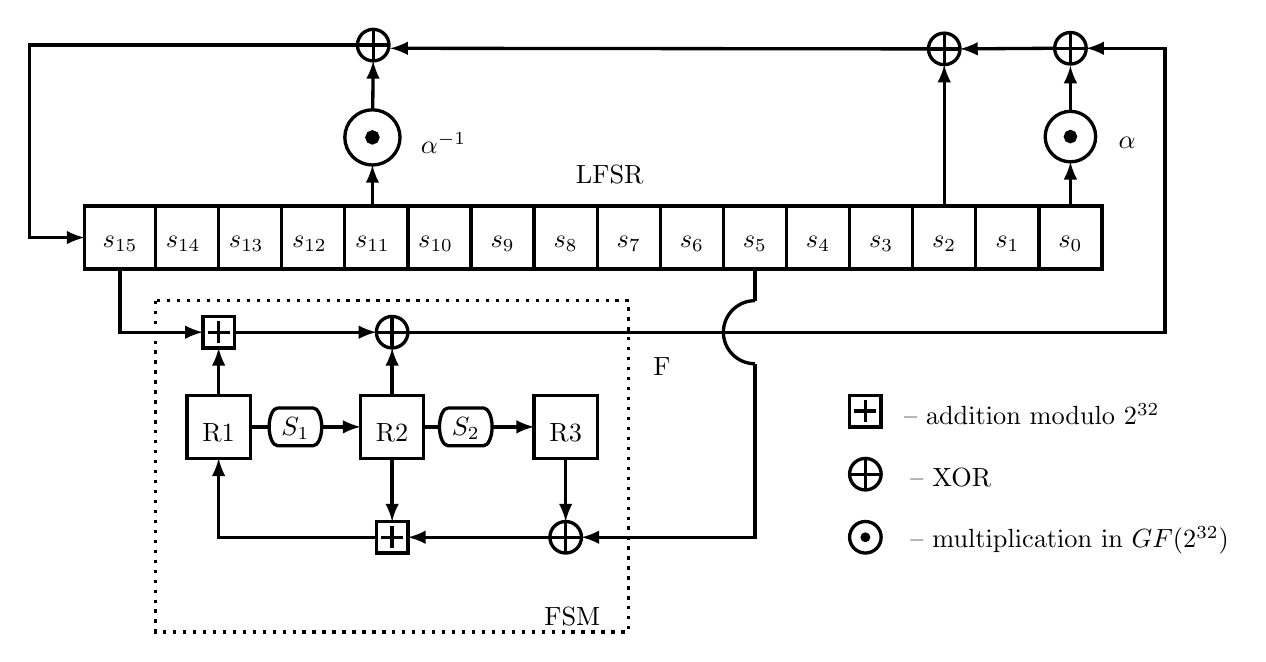
\begin{tikzpicture}[scale=0.95,every node/.style={scale=0.95}]
\pgftransformxscale{1.000000}
\pgftransformyscale{-1.000000}
\definecolor{dialinecolor}{rgb}{0.000000, 0.000000, 0.000000}
\pgfsetstrokecolor{dialinecolor}
\definecolor{dialinecolor}{rgb}{1.000000, 1.000000, 1.000000}
\pgfsetfillcolor{dialinecolor}
\definecolor{dialinecolor}{rgb}{1.000000, 1.000000, 1.000000}
\pgfsetfillcolor{dialinecolor}
\fill (40.000000\du,4.000000\du)--(40.000000\du,6.000000\du)--(42.000000\du,6.000000\du)--(42.000000\du,4.000000\du)--cycle;
\pgfsetlinewidth{0.100000\du}
\pgfsetdash{}{0pt}
\pgfsetdash{}{0pt}
\pgfsetmiterjoin
\definecolor{dialinecolor}{rgb}{0.000000, 0.000000, 0.000000}
\pgfsetstrokecolor{dialinecolor}
\draw (40.000000\du,4.000000\du)--(40.000000\du,6.000000\du)--(42.000000\du,6.000000\du)--(42.000000\du,4.000000\du)--cycle;
% setfont left to latex
\definecolor{dialinecolor}{rgb}{0.000000, 0.000000, 0.000000}
\pgfsetstrokecolor{dialinecolor}
\node at (41.000000\du,5.195000\du){$s_{0}$};
\definecolor{dialinecolor}{rgb}{1.000000, 1.000000, 1.000000}
\pgfsetfillcolor{dialinecolor}
\fill (38.000000\du,4.000000\du)--(38.000000\du,6.000000\du)--(40.000000\du,6.000000\du)--(40.000000\du,4.000000\du)--cycle;
\pgfsetlinewidth{0.100000\du}
\pgfsetdash{}{0pt}
\pgfsetdash{}{0pt}
\pgfsetmiterjoin
\definecolor{dialinecolor}{rgb}{0.000000, 0.000000, 0.000000}
\pgfsetstrokecolor{dialinecolor}
\draw (38.000000\du,4.000000\du)--(38.000000\du,6.000000\du)--(40.000000\du,6.000000\du)--(40.000000\du,4.000000\du)--cycle;
% setfont left to latex
\definecolor{dialinecolor}{rgb}{0.000000, 0.000000, 0.000000}
\pgfsetstrokecolor{dialinecolor}
\node at (39.000000\du,5.195000\du){$s_{1}$};
\definecolor{dialinecolor}{rgb}{1.000000, 1.000000, 1.000000}
\pgfsetfillcolor{dialinecolor}
\fill (36.000000\du,4.000000\du)--(36.000000\du,6.000000\du)--(38.000000\du,6.000000\du)--(38.000000\du,4.000000\du)--cycle;
\pgfsetlinewidth{0.100000\du}
\pgfsetdash{}{0pt}
\pgfsetdash{}{0pt}
\pgfsetmiterjoin
\definecolor{dialinecolor}{rgb}{0.000000, 0.000000, 0.000000}
\pgfsetstrokecolor{dialinecolor}
\draw (36.000000\du,4.000000\du)--(36.000000\du,6.000000\du)--(38.000000\du,6.000000\du)--(38.000000\du,4.000000\du)--cycle;
% setfont left to latex
\definecolor{dialinecolor}{rgb}{0.000000, 0.000000, 0.000000}
\pgfsetstrokecolor{dialinecolor}
\node at (37.000000\du,5.195000\du){$s_{2}$};
\definecolor{dialinecolor}{rgb}{1.000000, 1.000000, 1.000000}
\pgfsetfillcolor{dialinecolor}
\fill (34.000000\du,4.000000\du)--(34.000000\du,6.000000\du)--(36.000000\du,6.000000\du)--(36.000000\du,4.000000\du)--cycle;
\pgfsetlinewidth{0.100000\du}
\pgfsetdash{}{0pt}
\pgfsetdash{}{0pt}
\pgfsetmiterjoin
\definecolor{dialinecolor}{rgb}{0.000000, 0.000000, 0.000000}
\pgfsetstrokecolor{dialinecolor}
\draw (34.000000\du,4.000000\du)--(34.000000\du,6.000000\du)--(36.000000\du,6.000000\du)--(36.000000\du,4.000000\du)--cycle;
% setfont left to latex
\definecolor{dialinecolor}{rgb}{0.000000, 0.000000, 0.000000}
\pgfsetstrokecolor{dialinecolor}
\node at (35.000000\du,5.195000\du){$s_{3}$};
\definecolor{dialinecolor}{rgb}{1.000000, 1.000000, 1.000000}
\pgfsetfillcolor{dialinecolor}
\fill (32.000000\du,4.000000\du)--(32.000000\du,6.000000\du)--(34.000000\du,6.000000\du)--(34.000000\du,4.000000\du)--cycle;
\pgfsetlinewidth{0.100000\du}
\pgfsetdash{}{0pt}
\pgfsetdash{}{0pt}
\pgfsetmiterjoin
\definecolor{dialinecolor}{rgb}{0.000000, 0.000000, 0.000000}
\pgfsetstrokecolor{dialinecolor}
\draw (32.000000\du,4.000000\du)--(32.000000\du,6.000000\du)--(34.000000\du,6.000000\du)--(34.000000\du,4.000000\du)--cycle;
% setfont left to latex
\definecolor{dialinecolor}{rgb}{0.000000, 0.000000, 0.000000}
\pgfsetstrokecolor{dialinecolor}
\node at (33.000000\du,5.195000\du){$s_{4}$};
\definecolor{dialinecolor}{rgb}{1.000000, 1.000000, 1.000000}
\pgfsetfillcolor{dialinecolor}
\fill (30.000000\du,4.000000\du)--(30.000000\du,6.000000\du)--(32.000000\du,6.000000\du)--(32.000000\du,4.000000\du)--cycle;
\pgfsetlinewidth{0.100000\du}
\pgfsetdash{}{0pt}
\pgfsetdash{}{0pt}
\pgfsetmiterjoin
\definecolor{dialinecolor}{rgb}{0.000000, 0.000000, 0.000000}
\pgfsetstrokecolor{dialinecolor}
\draw (30.000000\du,4.000000\du)--(30.000000\du,6.000000\du)--(32.000000\du,6.000000\du)--(32.000000\du,4.000000\du)--cycle;
% setfont left to latex
\definecolor{dialinecolor}{rgb}{0.000000, 0.000000, 0.000000}
\pgfsetstrokecolor{dialinecolor}
\node at (31.000000\du,5.195000\du){$s_{5}$};
\definecolor{dialinecolor}{rgb}{1.000000, 1.000000, 1.000000}
\pgfsetfillcolor{dialinecolor}
\fill (28.000000\du,4.000000\du)--(28.000000\du,6.000000\du)--(30.000000\du,6.000000\du)--(30.000000\du,4.000000\du)--cycle;
\pgfsetlinewidth{0.100000\du}
\pgfsetdash{}{0pt}
\pgfsetdash{}{0pt}
\pgfsetmiterjoin
\definecolor{dialinecolor}{rgb}{0.000000, 0.000000, 0.000000}
\pgfsetstrokecolor{dialinecolor}
\draw (28.000000\du,4.000000\du)--(28.000000\du,6.000000\du)--(30.000000\du,6.000000\du)--(30.000000\du,4.000000\du)--cycle;
% setfont left to latex
\definecolor{dialinecolor}{rgb}{0.000000, 0.000000, 0.000000}
\pgfsetstrokecolor{dialinecolor}
\node at (29.000000\du,5.195000\du){$s_{6}$};
\definecolor{dialinecolor}{rgb}{1.000000, 1.000000, 1.000000}
\pgfsetfillcolor{dialinecolor}
\fill (26.000000\du,4.000000\du)--(26.000000\du,6.000000\du)--(28.000000\du,6.000000\du)--(28.000000\du,4.000000\du)--cycle;
\pgfsetlinewidth{0.100000\du}
\pgfsetdash{}{0pt}
\pgfsetdash{}{0pt}
\pgfsetmiterjoin
\definecolor{dialinecolor}{rgb}{0.000000, 0.000000, 0.000000}
\pgfsetstrokecolor{dialinecolor}
\draw (26.000000\du,4.000000\du)--(26.000000\du,6.000000\du)--(28.000000\du,6.000000\du)--(28.000000\du,4.000000\du)--cycle;
% setfont left to latex
\definecolor{dialinecolor}{rgb}{0.000000, 0.000000, 0.000000}
\pgfsetstrokecolor{dialinecolor}
\node at (27.000000\du,5.195000\du){$s_{7}$};
\definecolor{dialinecolor}{rgb}{1.000000, 1.000000, 1.000000}
\pgfsetfillcolor{dialinecolor}
\fill (24.000000\du,4.000000\du)--(24.000000\du,6.000000\du)--(26.000000\du,6.000000\du)--(26.000000\du,4.000000\du)--cycle;
\pgfsetlinewidth{0.100000\du}
\pgfsetdash{}{0pt}
\pgfsetdash{}{0pt}
\pgfsetmiterjoin
\definecolor{dialinecolor}{rgb}{0.000000, 0.000000, 0.000000}
\pgfsetstrokecolor{dialinecolor}
\draw (24.000000\du,4.000000\du)--(24.000000\du,6.000000\du)--(26.000000\du,6.000000\du)--(26.000000\du,4.000000\du)--cycle;
% setfont left to latex
\definecolor{dialinecolor}{rgb}{0.000000, 0.000000, 0.000000}
\pgfsetstrokecolor{dialinecolor}
\node at (25.000000\du,5.195000\du){$s_{8}$};
\definecolor{dialinecolor}{rgb}{1.000000, 1.000000, 1.000000}
\pgfsetfillcolor{dialinecolor}
\fill (22.000000\du,4.000000\du)--(22.000000\du,6.000000\du)--(24.000000\du,6.000000\du)--(24.000000\du,4.000000\du)--cycle;
\pgfsetlinewidth{0.100000\du}
\pgfsetdash{}{0pt}
\pgfsetdash{}{0pt}
\pgfsetmiterjoin
\definecolor{dialinecolor}{rgb}{0.000000, 0.000000, 0.000000}
\pgfsetstrokecolor{dialinecolor}
\draw (22.000000\du,4.000000\du)--(22.000000\du,6.000000\du)--(24.000000\du,6.000000\du)--(24.000000\du,4.000000\du)--cycle;
% setfont left to latex
\definecolor{dialinecolor}{rgb}{0.000000, 0.000000, 0.000000}
\pgfsetstrokecolor{dialinecolor}
\node at (23.000000\du,5.195000\du){$s_{9}$};
\definecolor{dialinecolor}{rgb}{1.000000, 1.000000, 1.000000}
\pgfsetfillcolor{dialinecolor}
\fill (19.750000\du,4.000000\du)--(19.750000\du,6.000000\du)--(22.000000\du,6.000000\du)--(22.000000\du,4.000000\du)--cycle;
\pgfsetlinewidth{0.100000\du}
\pgfsetdash{}{0pt}
\pgfsetdash{}{0pt}
\pgfsetmiterjoin
\definecolor{dialinecolor}{rgb}{0.000000, 0.000000, 0.000000}
\pgfsetstrokecolor{dialinecolor}
\draw (19.750000\du,4.000000\du)--(19.750000\du,6.000000\du)--(22.000000\du,6.000000\du)--(22.000000\du,4.000000\du)--cycle;
% setfont left to latex
\definecolor{dialinecolor}{rgb}{0.000000, 0.000000, 0.000000}
\pgfsetstrokecolor{dialinecolor}
\node at (20.875000\du,5.195000\du){$s_{10}$};
\definecolor{dialinecolor}{rgb}{1.000000, 1.000000, 1.000000}
\pgfsetfillcolor{dialinecolor}
\fill (17.750000\du,4.000000\du)--(17.750000\du,6.000000\du)--(20.000000\du,6.000000\du)--(20.000000\du,4.000000\du)--cycle;
\pgfsetlinewidth{0.100000\du}
\pgfsetdash{}{0pt}
\pgfsetdash{}{0pt}
\pgfsetmiterjoin
\definecolor{dialinecolor}{rgb}{0.000000, 0.000000, 0.000000}
\pgfsetstrokecolor{dialinecolor}
\draw (17.750000\du,4.000000\du)--(17.750000\du,6.000000\du)--(20.000000\du,6.000000\du)--(20.000000\du,4.000000\du)--cycle;
% setfont left to latex
\definecolor{dialinecolor}{rgb}{0.000000, 0.000000, 0.000000}
\pgfsetstrokecolor{dialinecolor}
\node at (18.875000\du,5.195000\du){$s_{11}$};
\definecolor{dialinecolor}{rgb}{1.000000, 1.000000, 1.000000}
\pgfsetfillcolor{dialinecolor}
\fill (15.750000\du,4.000000\du)--(15.750000\du,6.000000\du)--(18.000000\du,6.000000\du)--(18.000000\du,4.000000\du)--cycle;
\pgfsetlinewidth{0.100000\du}
\pgfsetdash{}{0pt}
\pgfsetdash{}{0pt}
\pgfsetmiterjoin
\definecolor{dialinecolor}{rgb}{0.000000, 0.000000, 0.000000}
\pgfsetstrokecolor{dialinecolor}
\draw (15.750000\du,4.000000\du)--(15.750000\du,6.000000\du)--(18.000000\du,6.000000\du)--(18.000000\du,4.000000\du)--cycle;
% setfont left to latex
\definecolor{dialinecolor}{rgb}{0.000000, 0.000000, 0.000000}
\pgfsetstrokecolor{dialinecolor}
\node at (16.875000\du,5.195000\du){$s_{12}$};
\definecolor{dialinecolor}{rgb}{1.000000, 1.000000, 1.000000}
\pgfsetfillcolor{dialinecolor}
\fill (13.750000\du,4.000000\du)--(13.750000\du,6.000000\du)--(16.000000\du,6.000000\du)--(16.000000\du,4.000000\du)--cycle;
\pgfsetlinewidth{0.100000\du}
\pgfsetdash{}{0pt}
\pgfsetdash{}{0pt}
\pgfsetmiterjoin
\definecolor{dialinecolor}{rgb}{0.000000, 0.000000, 0.000000}
\pgfsetstrokecolor{dialinecolor}
\draw (13.750000\du,4.000000\du)--(13.750000\du,6.000000\du)--(16.000000\du,6.000000\du)--(16.000000\du,4.000000\du)--cycle;
% setfont left to latex
\definecolor{dialinecolor}{rgb}{0.000000, 0.000000, 0.000000}
\pgfsetstrokecolor{dialinecolor}
\node at (14.875000\du,5.195000\du){$s_{13}$};
\definecolor{dialinecolor}{rgb}{1.000000, 1.000000, 1.000000}
\pgfsetfillcolor{dialinecolor}
\fill (11.750000\du,4.000000\du)--(11.750000\du,6.000000\du)--(14.000000\du,6.000000\du)--(14.000000\du,4.000000\du)--cycle;
\pgfsetlinewidth{0.100000\du}
\pgfsetdash{}{0pt}
\pgfsetdash{}{0pt}
\pgfsetmiterjoin
\definecolor{dialinecolor}{rgb}{0.000000, 0.000000, 0.000000}
\pgfsetstrokecolor{dialinecolor}
\draw (11.750000\du,4.000000\du)--(11.750000\du,6.000000\du)--(14.000000\du,6.000000\du)--(14.000000\du,4.000000\du)--cycle;
% setfont left to latex
\definecolor{dialinecolor}{rgb}{0.000000, 0.000000, 0.000000}
\pgfsetstrokecolor{dialinecolor}
\node at (12.875000\du,5.195000\du){$s_{14}$};
\definecolor{dialinecolor}{rgb}{1.000000, 1.000000, 1.000000}
\pgfsetfillcolor{dialinecolor}
\fill (9.750000\du,4.000000\du)--(9.750000\du,6.000000\du)--(12.000000\du,6.000000\du)--(12.000000\du,4.000000\du)--cycle;
\pgfsetlinewidth{0.100000\du}
\pgfsetdash{}{0pt}
\pgfsetdash{}{0pt}
\pgfsetmiterjoin
\definecolor{dialinecolor}{rgb}{0.000000, 0.000000, 0.000000}
\pgfsetstrokecolor{dialinecolor}
\draw (9.750000\du,4.000000\du)--(9.750000\du,6.000000\du)--(12.000000\du,6.000000\du)--(12.000000\du,4.000000\du)--cycle;
% setfont left to latex
\definecolor{dialinecolor}{rgb}{0.000000, 0.000000, 0.000000}
\pgfsetstrokecolor{dialinecolor}
\node at (10.875000\du,5.195000\du){$s_{15}$};
\definecolor{dialinecolor}{rgb}{1.000000, 1.000000, 1.000000}
\pgfsetfillcolor{dialinecolor}
\fill (13.000000\du,10.000000\du)--(13.000000\du,12.000000\du)--(15.000000\du,12.000000\du)--(15.000000\du,10.000000\du)--cycle;
\pgfsetlinewidth{0.100000\du}
\pgfsetdash{}{0pt}
\pgfsetdash{}{0pt}
\pgfsetmiterjoin
\definecolor{dialinecolor}{rgb}{0.000000, 0.000000, 0.000000}
\pgfsetstrokecolor{dialinecolor}
\draw (13.000000\du,10.000000\du)--(13.000000\du,12.000000\du)--(15.000000\du,12.000000\du)--(15.000000\du,10.000000\du)--cycle;
% setfont left to latex
\definecolor{dialinecolor}{rgb}{0.000000, 0.000000, 0.000000}
\pgfsetstrokecolor{dialinecolor}
\node at (14.000000\du,11.195000\du){R1};
\definecolor{dialinecolor}{rgb}{1.000000, 1.000000, 1.000000}
\pgfsetfillcolor{dialinecolor}
\fill (18.500000\du,10.000000\du)--(18.500000\du,12.000000\du)--(20.500000\du,12.000000\du)--(20.500000\du,10.000000\du)--cycle;
\pgfsetlinewidth{0.100000\du}
\pgfsetdash{}{0pt}
\pgfsetdash{}{0pt}
\pgfsetmiterjoin
\definecolor{dialinecolor}{rgb}{0.000000, 0.000000, 0.000000}
\pgfsetstrokecolor{dialinecolor}
\draw (18.500000\du,10.000000\du)--(18.500000\du,12.000000\du)--(20.500000\du,12.000000\du)--(20.500000\du,10.000000\du)--cycle;
% setfont left to latex
\definecolor{dialinecolor}{rgb}{0.000000, 0.000000, 0.000000}
\pgfsetstrokecolor{dialinecolor}
\node at (19.500000\du,11.195000\du){R2};
\definecolor{dialinecolor}{rgb}{1.000000, 1.000000, 1.000000}
\pgfsetfillcolor{dialinecolor}
\fill (24.000000\du,10.000000\du)--(24.000000\du,12.000000\du)--(26.000000\du,12.000000\du)--(26.000000\du,10.000000\du)--cycle;
\pgfsetlinewidth{0.100000\du}
\pgfsetdash{}{0pt}
\pgfsetdash{}{0pt}
\pgfsetmiterjoin
\definecolor{dialinecolor}{rgb}{0.000000, 0.000000, 0.000000}
\pgfsetstrokecolor{dialinecolor}
\draw (24.000000\du,10.000000\du)--(24.000000\du,12.000000\du)--(26.000000\du,12.000000\du)--(26.000000\du,10.000000\du)--cycle;
% setfont left to latex
\definecolor{dialinecolor}{rgb}{0.000000, 0.000000, 0.000000}
\pgfsetstrokecolor{dialinecolor}
\node at (25.000000\du,11.195000\du){R3};
\pgfsetlinewidth{0.100000\du}
\pgfsetdash{}{0pt}
\pgfsetdash{}{0pt}
\pgfsetbuttcap
\pgfsetmiterjoin
\pgfsetlinewidth{0.100000\du}
\pgfsetbuttcap
\pgfsetmiterjoin
\pgfsetdash{}{0pt}
\definecolor{dialinecolor}{rgb}{1.000000, 1.000000, 1.000000}
\pgfsetfillcolor{dialinecolor}
\pgfpathellipse{\pgfpoint{41.000000\du}{1.800000\du}}{\pgfpoint{0.800000\du}{0\du}}{\pgfpoint{0\du}{0.800000\du}}
\pgfusepath{fill}
\definecolor{dialinecolor}{rgb}{0.000000, 0.000000, 0.000000}
\pgfsetstrokecolor{dialinecolor}
\pgfpathellipse{\pgfpoint{41.000000\du}{1.800000\du}}{\pgfpoint{0.800000\du}{0\du}}{\pgfpoint{0\du}{0.800000\du}}
\pgfusepath{stroke}
\pgfsetbuttcap
\pgfsetmiterjoin
\pgfsetdash{}{0pt}
\definecolor{dialinecolor}{rgb}{0.000000, 0.000000, 0.000000}
\pgfsetfillcolor{dialinecolor}
\pgfpathellipse{\pgfpoint{41.000000\du}{1.800000\du}}{\pgfpoint{0.160000\du}{0\du}}{\pgfpoint{0\du}{0.160000\du}}
\pgfusepath{fill}
\definecolor{dialinecolor}{rgb}{0.000000, 0.000000, 0.000000}
\pgfsetstrokecolor{dialinecolor}
\pgfpathellipse{\pgfpoint{41.000000\du}{1.800000\du}}{\pgfpoint{0.160000\du}{0\du}}{\pgfpoint{0\du}{0.160000\du}}
\pgfusepath{stroke}
\pgfsetlinewidth{0.100000\du}
\pgfsetdash{}{0pt}
\pgfsetdash{}{0pt}
\pgfsetbuttcap
\pgfsetmiterjoin
\pgfsetlinewidth{0.100000\du}
\pgfsetbuttcap
\pgfsetmiterjoin
\pgfsetdash{}{0pt}
\definecolor{dialinecolor}{rgb}{1.000000, 1.000000, 1.000000}
\pgfsetfillcolor{dialinecolor}
\pgfpathellipse{\pgfpoint{41.000000\du}{-1.000000\du}}{\pgfpoint{0.500000\du}{0\du}}{\pgfpoint{0\du}{0.500000\du}}
\pgfusepath{fill}
\definecolor{dialinecolor}{rgb}{0.000000, 0.000000, 0.000000}
\pgfsetstrokecolor{dialinecolor}
\pgfpathellipse{\pgfpoint{41.000000\du}{-1.000000\du}}{\pgfpoint{0.500000\du}{0\du}}{\pgfpoint{0\du}{0.500000\du}}
\pgfusepath{stroke}
\pgfsetbuttcap
\pgfsetmiterjoin
\pgfsetdash{}{0pt}
\definecolor{dialinecolor}{rgb}{0.000000, 0.000000, 0.000000}
\pgfsetstrokecolor{dialinecolor}
\draw (41.000000\du,-1.500000\du)--(41.000000\du,-0.500000\du);
\pgfsetbuttcap
\pgfsetmiterjoin
\pgfsetdash{}{0pt}
\definecolor{dialinecolor}{rgb}{0.000000, 0.000000, 0.000000}
\pgfsetstrokecolor{dialinecolor}
\draw (40.500000\du,-1.000000\du)--(41.500000\du,-1.000000\du);
\pgfsetlinewidth{0.100000\du}
\pgfsetdash{}{0pt}
\pgfsetdash{}{0pt}
\pgfsetbuttcap
\pgfsetmiterjoin
\pgfsetlinewidth{0.100000\du}
\pgfsetbuttcap
\pgfsetmiterjoin
\pgfsetdash{}{0pt}
\definecolor{dialinecolor}{rgb}{1.000000, 1.000000, 1.000000}
\pgfsetfillcolor{dialinecolor}
\pgfpathellipse{\pgfpoint{37.000000\du}{-0.980000\du}}{\pgfpoint{0.500000\du}{0\du}}{\pgfpoint{0\du}{0.500000\du}}
\pgfusepath{fill}
\definecolor{dialinecolor}{rgb}{0.000000, 0.000000, 0.000000}
\pgfsetstrokecolor{dialinecolor}
\pgfpathellipse{\pgfpoint{37.000000\du}{-0.980000\du}}{\pgfpoint{0.500000\du}{0\du}}{\pgfpoint{0\du}{0.500000\du}}
\pgfusepath{stroke}
\pgfsetbuttcap
\pgfsetmiterjoin
\pgfsetdash{}{0pt}
\definecolor{dialinecolor}{rgb}{0.000000, 0.000000, 0.000000}
\pgfsetstrokecolor{dialinecolor}
\draw (37.000000\du,-1.480000\du)--(37.000000\du,-0.480000\du);
\pgfsetbuttcap
\pgfsetmiterjoin
\pgfsetdash{}{0pt}
\definecolor{dialinecolor}{rgb}{0.000000, 0.000000, 0.000000}
\pgfsetstrokecolor{dialinecolor}
\draw (36.500000\du,-0.980000\du)--(37.500000\du,-0.980000\du);
\pgfsetlinewidth{0.100000\du}
\pgfsetdash{}{0pt}
\pgfsetdash{}{0pt}
\pgfsetbuttcap
\pgfsetmiterjoin
\pgfsetlinewidth{0.100000\du}
\pgfsetbuttcap
\pgfsetmiterjoin
\pgfsetdash{}{0pt}
\definecolor{dialinecolor}{rgb}{1.000000, 1.000000, 1.000000}
\pgfsetfillcolor{dialinecolor}
\pgfpathellipse{\pgfpoint{18.900000\du}{-1.100000\du}}{\pgfpoint{0.500000\du}{0\du}}{\pgfpoint{0\du}{0.500000\du}}
\pgfusepath{fill}
\definecolor{dialinecolor}{rgb}{0.000000, 0.000000, 0.000000}
\pgfsetstrokecolor{dialinecolor}
\pgfpathellipse{\pgfpoint{18.900000\du}{-1.100000\du}}{\pgfpoint{0.500000\du}{0\du}}{\pgfpoint{0\du}{0.500000\du}}
\pgfusepath{stroke}
\pgfsetbuttcap
\pgfsetmiterjoin
\pgfsetdash{}{0pt}
\definecolor{dialinecolor}{rgb}{0.000000, 0.000000, 0.000000}
\pgfsetstrokecolor{dialinecolor}
\draw (18.900000\du,-1.600000\du)--(18.900000\du,-0.600000\du);
\pgfsetbuttcap
\pgfsetmiterjoin
\pgfsetdash{}{0pt}
\definecolor{dialinecolor}{rgb}{0.000000, 0.000000, 0.000000}
\pgfsetstrokecolor{dialinecolor}
\draw (18.400000\du,-1.100000\du)--(19.400000\du,-1.100000\du);
\pgfsetlinewidth{0.100000\du}
\pgfsetdash{}{0pt}
\pgfsetdash{}{0pt}
\pgfsetbuttcap
\pgfsetmiterjoin
\pgfsetlinewidth{0.100000\du}
\pgfsetbuttcap
\pgfsetmiterjoin
\pgfsetdash{}{0pt}
\definecolor{dialinecolor}{rgb}{1.000000, 1.000000, 1.000000}
\pgfsetfillcolor{dialinecolor}
\fill (13.500000\du,7.500000\du)--(13.500000\du,8.500000\du)--(14.500000\du,8.500000\du)--(14.500000\du,7.500000\du)--cycle;
\definecolor{dialinecolor}{rgb}{0.000000, 0.000000, 0.000000}
\pgfsetstrokecolor{dialinecolor}
\draw (13.500000\du,7.500000\du)--(13.500000\du,8.500000\du)--(14.500000\du,8.500000\du)--(14.500000\du,7.500000\du)--cycle;
\pgfsetbuttcap
\pgfsetmiterjoin
\pgfsetdash{}{0pt}
\definecolor{dialinecolor}{rgb}{0.000000, 0.000000, 0.000000}
\pgfsetstrokecolor{dialinecolor}
\draw (14.000000\du,7.650000\du)--(14.000000\du,8.350000\du);
\pgfsetbuttcap
\pgfsetmiterjoin
\pgfsetdash{}{0pt}
\definecolor{dialinecolor}{rgb}{0.000000, 0.000000, 0.000000}
\pgfsetstrokecolor{dialinecolor}
\draw (13.650000\du,8.000000\du)--(14.350000\du,8.000000\du);
\pgfsetlinewidth{0.100000\du}
\pgfsetdash{}{0pt}
\pgfsetdash{}{0pt}
\pgfsetbuttcap
\pgfsetmiterjoin
\pgfsetlinewidth{0.100000\du}
\pgfsetbuttcap
\pgfsetmiterjoin
\pgfsetdash{}{0pt}
\definecolor{dialinecolor}{rgb}{1.000000, 1.000000, 1.000000}
\pgfsetfillcolor{dialinecolor}
\fill (19.000000\du,14.000000\du)--(19.000000\du,15.000000\du)--(20.000000\du,15.000000\du)--(20.000000\du,14.000000\du)--cycle;
\definecolor{dialinecolor}{rgb}{0.000000, 0.000000, 0.000000}
\pgfsetstrokecolor{dialinecolor}
\draw (19.000000\du,14.000000\du)--(19.000000\du,15.000000\du)--(20.000000\du,15.000000\du)--(20.000000\du,14.000000\du)--cycle;
\pgfsetbuttcap
\pgfsetmiterjoin
\pgfsetdash{}{0pt}
\definecolor{dialinecolor}{rgb}{0.000000, 0.000000, 0.000000}
\pgfsetstrokecolor{dialinecolor}
\draw (19.500000\du,14.150000\du)--(19.500000\du,14.850000\du);
\pgfsetbuttcap
\pgfsetmiterjoin
\pgfsetdash{}{0pt}
\definecolor{dialinecolor}{rgb}{0.000000, 0.000000, 0.000000}
\pgfsetstrokecolor{dialinecolor}
\draw (19.150000\du,14.500000\du)--(19.850000\du,14.500000\du);
\pgfsetlinewidth{0.100000\du}
\pgfsetdash{}{0pt}
\pgfsetdash{}{0pt}
\pgfsetbuttcap
\pgfsetmiterjoin
\pgfsetlinewidth{0.100000\du}
\pgfsetbuttcap
\pgfsetmiterjoin
\pgfsetdash{}{0pt}
\definecolor{dialinecolor}{rgb}{1.000000, 1.000000, 1.000000}
\pgfsetfillcolor{dialinecolor}
\pgfpathellipse{\pgfpoint{25.000000\du}{14.500000\du}}{\pgfpoint{0.500000\du}{0\du}}{\pgfpoint{0\du}{0.500000\du}}
\pgfusepath{fill}
\definecolor{dialinecolor}{rgb}{0.000000, 0.000000, 0.000000}
\pgfsetstrokecolor{dialinecolor}
\pgfpathellipse{\pgfpoint{25.000000\du}{14.500000\du}}{\pgfpoint{0.500000\du}{0\du}}{\pgfpoint{0\du}{0.500000\du}}
\pgfusepath{stroke}
\pgfsetbuttcap
\pgfsetmiterjoin
\pgfsetdash{}{0pt}
\definecolor{dialinecolor}{rgb}{0.000000, 0.000000, 0.000000}
\pgfsetstrokecolor{dialinecolor}
\draw (25.000000\du,14.000000\du)--(25.000000\du,15.000000\du);
\pgfsetbuttcap
\pgfsetmiterjoin
\pgfsetdash{}{0pt}
\definecolor{dialinecolor}{rgb}{0.000000, 0.000000, 0.000000}
\pgfsetstrokecolor{dialinecolor}
\draw (24.500000\du,14.500000\du)--(25.500000\du,14.500000\du);
\pgfsetlinewidth{0.100000\du}
\pgfsetdash{}{0pt}
\pgfsetdash{}{0pt}
\pgfsetbuttcap
\pgfsetmiterjoin
\pgfsetlinewidth{0.100000\du}
\pgfsetbuttcap
\pgfsetmiterjoin
\pgfsetdash{}{0pt}
\definecolor{dialinecolor}{rgb}{1.000000, 1.000000, 1.000000}
\pgfsetfillcolor{dialinecolor}
\pgfpathellipse{\pgfpoint{19.500000\du}{8.000000\du}}{\pgfpoint{0.500000\du}{0\du}}{\pgfpoint{0\du}{0.500000\du}}
\pgfusepath{fill}
\definecolor{dialinecolor}{rgb}{0.000000, 0.000000, 0.000000}
\pgfsetstrokecolor{dialinecolor}
\pgfpathellipse{\pgfpoint{19.500000\du}{8.000000\du}}{\pgfpoint{0.500000\du}{0\du}}{\pgfpoint{0\du}{0.500000\du}}
\pgfusepath{stroke}
\pgfsetbuttcap
\pgfsetmiterjoin
\pgfsetdash{}{0pt}
\definecolor{dialinecolor}{rgb}{0.000000, 0.000000, 0.000000}
\pgfsetstrokecolor{dialinecolor}
\draw (19.500000\du,7.500000\du)--(19.500000\du,8.500000\du);
\pgfsetbuttcap
\pgfsetmiterjoin
\pgfsetdash{}{0pt}
\definecolor{dialinecolor}{rgb}{0.000000, 0.000000, 0.000000}
\pgfsetstrokecolor{dialinecolor}
\draw (19.000000\du,8.000000\du)--(20.000000\du,8.000000\du);
\pgfsetlinewidth{0.100000\du}
\pgfsetdash{}{0pt}
\pgfsetdash{}{0pt}
\pgfsetbuttcap
{
\definecolor{dialinecolor}{rgb}{0.000000, 0.000000, 0.000000}
\pgfsetfillcolor{dialinecolor}
% was here!!!
\pgfsetarrowsend{latex}
\definecolor{dialinecolor}{rgb}{0.000000, 0.000000, 0.000000}
\pgfsetstrokecolor{dialinecolor}
\draw (14.500000\du,8.000000\du)--(19.000000\du,8.000000\du);
}
\pgfsetlinewidth{0.100000\du}
\pgfsetdash{}{0pt}
\pgfsetdash{}{0pt}
\pgfsetbuttcap
{
\definecolor{dialinecolor}{rgb}{0.000000, 0.000000, 0.000000}
\pgfsetfillcolor{dialinecolor}
% was here!!!
\pgfsetarrowsend{latex}
\definecolor{dialinecolor}{rgb}{0.000000, 0.000000, 0.000000}
\pgfsetstrokecolor{dialinecolor}
\draw (14.000000\du,9.949890\du)--(14.000000\du,8.500000\du);
}
\pgfsetlinewidth{0.100000\du}
\pgfsetdash{}{0pt}
\pgfsetdash{}{0pt}
\pgfsetbuttcap
{
\definecolor{dialinecolor}{rgb}{0.000000, 0.000000, 0.000000}
\pgfsetfillcolor{dialinecolor}
% was here!!!
\pgfsetarrowsend{latex}
\definecolor{dialinecolor}{rgb}{0.000000, 0.000000, 0.000000}
\pgfsetstrokecolor{dialinecolor}
\draw (15.000000\du,11.000000\du)--(18.500000\du,11.000000\du);
}
\pgfsetlinewidth{0.100000\du}
\pgfsetdash{}{0pt}
\pgfsetdash{}{0pt}
\pgfsetbuttcap
\pgfsetmiterjoin
\pgfsetlinewidth{0.100000\du}
\pgfsetbuttcap
\pgfsetmiterjoin
\pgfsetdash{}{0pt}
\definecolor{dialinecolor}{rgb}{1.000000, 1.000000, 1.000000}
\pgfsetfillcolor{dialinecolor}
\pgfpathmoveto{\pgfpoint{15.878125\du}{10.400000\du}}
\pgfpathlineto{\pgfpoint{16.990625\du}{10.400000\du}}
\pgfpathcurveto{\pgfpoint{17.144229\du}{10.400000\du}}{\pgfpoint{17.268750\du}{10.668629\du}}{\pgfpoint{17.268750\du}{11.000000\du}}
\pgfpathcurveto{\pgfpoint{17.268750\du}{11.331371\du}}{\pgfpoint{17.144229\du}{11.600000\du}}{\pgfpoint{16.990625\du}{11.600000\du}}
\pgfpathlineto{\pgfpoint{15.878125\du}{11.600000\du}}
\pgfpathcurveto{\pgfpoint{15.724521\du}{11.600000\du}}{\pgfpoint{15.600000\du}{11.331371\du}}{\pgfpoint{15.600000\du}{11.000000\du}}
\pgfpathcurveto{\pgfpoint{15.600000\du}{10.668629\du}}{\pgfpoint{15.724521\du}{10.400000\du}}{\pgfpoint{15.878125\du}{10.400000\du}}
\pgfusepath{fill}
\definecolor{dialinecolor}{rgb}{0.000000, 0.000000, 0.000000}
\pgfsetstrokecolor{dialinecolor}
\pgfpathmoveto{\pgfpoint{15.878125\du}{10.400000\du}}
\pgfpathlineto{\pgfpoint{16.990625\du}{10.400000\du}}
\pgfpathcurveto{\pgfpoint{17.144229\du}{10.400000\du}}{\pgfpoint{17.268750\du}{10.668629\du}}{\pgfpoint{17.268750\du}{11.000000\du}}
\pgfpathcurveto{\pgfpoint{17.268750\du}{11.331371\du}}{\pgfpoint{17.144229\du}{11.600000\du}}{\pgfpoint{16.990625\du}{11.600000\du}}
\pgfpathlineto{\pgfpoint{15.878125\du}{11.600000\du}}
\pgfpathcurveto{\pgfpoint{15.724521\du}{11.600000\du}}{\pgfpoint{15.600000\du}{11.331371\du}}{\pgfpoint{15.600000\du}{11.000000\du}}
\pgfpathcurveto{\pgfpoint{15.600000\du}{10.668629\du}}{\pgfpoint{15.724521\du}{10.400000\du}}{\pgfpoint{15.878125\du}{10.400000\du}}
\pgfusepath{stroke}
% setfont left to latex
\definecolor{dialinecolor}{rgb}{0.000000, 0.000000, 0.000000}
\pgfsetstrokecolor{dialinecolor}
\node at (16.434375\du,11.05\du){$S_{1}$};
\pgfsetlinewidth{0.100000\du}
\pgfsetdash{}{0pt}
\pgfsetdash{}{0pt}
\pgfsetbuttcap
{
\definecolor{dialinecolor}{rgb}{0.000000, 0.000000, 0.000000}
\pgfsetfillcolor{dialinecolor}
% was here!!!
\pgfsetarrowsend{latex}
\definecolor{dialinecolor}{rgb}{0.000000, 0.000000, 0.000000}
\pgfsetstrokecolor{dialinecolor}
\draw (20.500000\du,11.000000\du)--(24.000000\du,11.000000\du);
}
\pgfsetlinewidth{0.100000\du}
\pgfsetdash{}{0pt}
\pgfsetdash{}{0pt}
\pgfsetbuttcap
\pgfsetmiterjoin
\pgfsetlinewidth{0.100000\du}
\pgfsetbuttcap
\pgfsetmiterjoin
\pgfsetdash{}{0pt}
\definecolor{dialinecolor}{rgb}{1.000000, 1.000000, 1.000000}
\pgfsetfillcolor{dialinecolor}
\pgfpathmoveto{\pgfpoint{21.278125\du}{10.400000\du}}
\pgfpathlineto{\pgfpoint{22.390625\du}{10.400000\du}}
\pgfpathcurveto{\pgfpoint{22.544229\du}{10.400000\du}}{\pgfpoint{22.668750\du}{10.668629\du}}{\pgfpoint{22.668750\du}{11.000000\du}}
\pgfpathcurveto{\pgfpoint{22.668750\du}{11.331371\du}}{\pgfpoint{22.544229\du}{11.600000\du}}{\pgfpoint{22.390625\du}{11.600000\du}}
\pgfpathlineto{\pgfpoint{21.278125\du}{11.600000\du}}
\pgfpathcurveto{\pgfpoint{21.124521\du}{11.600000\du}}{\pgfpoint{21.000000\du}{11.331371\du}}{\pgfpoint{21.000000\du}{11.000000\du}}
\pgfpathcurveto{\pgfpoint{21.000000\du}{10.668629\du}}{\pgfpoint{21.124521\du}{10.400000\du}}{\pgfpoint{21.278125\du}{10.400000\du}}
\pgfusepath{fill}
\definecolor{dialinecolor}{rgb}{0.000000, 0.000000, 0.000000}
\pgfsetstrokecolor{dialinecolor}
\pgfpathmoveto{\pgfpoint{21.278125\du}{10.400000\du}}
\pgfpathlineto{\pgfpoint{22.390625\du}{10.400000\du}}
\pgfpathcurveto{\pgfpoint{22.544229\du}{10.400000\du}}{\pgfpoint{22.668750\du}{10.668629\du}}{\pgfpoint{22.668750\du}{11.000000\du}}
\pgfpathcurveto{\pgfpoint{22.668750\du}{11.331371\du}}{\pgfpoint{22.544229\du}{11.600000\du}}{\pgfpoint{22.390625\du}{11.600000\du}}
\pgfpathlineto{\pgfpoint{21.278125\du}{11.600000\du}}
\pgfpathcurveto{\pgfpoint{21.124521\du}{11.600000\du}}{\pgfpoint{21.000000\du}{11.331371\du}}{\pgfpoint{21.000000\du}{11.000000\du}}
\pgfpathcurveto{\pgfpoint{21.000000\du}{10.668629\du}}{\pgfpoint{21.124521\du}{10.400000\du}}{\pgfpoint{21.278125\du}{10.400000\du}}
\pgfusepath{stroke}
% setfont left to latex
\definecolor{dialinecolor}{rgb}{0.000000, 0.000000, 0.000000}
\pgfsetstrokecolor{dialinecolor}
\node at (21.834375\du,11.05\du){$S_{2}$};
\pgfsetlinewidth{0.100000\du}
\pgfsetdash{}{0pt}
\pgfsetdash{}{0pt}
\pgfsetbuttcap
{
\definecolor{dialinecolor}{rgb}{0.000000, 0.000000, 0.000000}
\pgfsetfillcolor{dialinecolor}
% was here!!!
\pgfsetarrowsend{latex}
\definecolor{dialinecolor}{rgb}{0.000000, 0.000000, 0.000000}
\pgfsetstrokecolor{dialinecolor}
\draw (19.500000\du,12.000000\du)--(19.500000\du,14.000000\du);
}
\pgfsetlinewidth{0.100000\du}
\pgfsetdash{}{0pt}
\pgfsetdash{}{0pt}
\pgfsetbuttcap
{
\definecolor{dialinecolor}{rgb}{0.000000, 0.000000, 0.000000}
\pgfsetfillcolor{dialinecolor}
% was here!!!
\pgfsetarrowsend{latex}
\definecolor{dialinecolor}{rgb}{0.000000, 0.000000, 0.000000}
\pgfsetstrokecolor{dialinecolor}
\draw (25.000000\du,12.000000\du)--(25.000000\du,14.000000\du);
}
\pgfsetlinewidth{0.100000\du}
\pgfsetdash{}{0pt}
\pgfsetdash{}{0pt}
\pgfsetbuttcap
{
\definecolor{dialinecolor}{rgb}{0.000000, 0.000000, 0.000000}
\pgfsetfillcolor{dialinecolor}
% was here!!!
\pgfsetarrowsend{latex}
\definecolor{dialinecolor}{rgb}{0.000000, 0.000000, 0.000000}
\pgfsetstrokecolor{dialinecolor}
\draw (24.500000\du,14.500000\du)--(20.000000\du,14.500000\du);
}
\pgfsetlinewidth{0.100000\du}
\pgfsetdash{}{0pt}
\pgfsetdash{}{0pt}
\pgfsetmiterjoin
\pgfsetbuttcap
{
\definecolor{dialinecolor}{rgb}{0.000000, 0.000000, 0.000000}
\pgfsetfillcolor{dialinecolor}
% was here!!!
\pgfsetarrowsend{latex}
{\pgfsetcornersarced{\pgfpoint{0.000000\du}{0.000000\du}}\definecolor{dialinecolor}{rgb}{0.000000, 0.000000, 0.000000}
\pgfsetstrokecolor{dialinecolor}
\draw (19.000000\du,14.500000\du)--(14.000000\du,14.500000\du)--(14.000000\du,12.000000\du);
}}
\pgfsetlinewidth{0.100000\du}
\pgfsetdash{}{0pt}
\pgfsetdash{}{0pt}
\pgfsetbuttcap
{
\definecolor{dialinecolor}{rgb}{0.000000, 0.000000, 0.000000}
\pgfsetfillcolor{dialinecolor}
% was here!!!
\pgfsetarrowsend{latex}
\definecolor{dialinecolor}{rgb}{0.000000, 0.000000, 0.000000}
\pgfsetstrokecolor{dialinecolor}
\draw (19.500000\du,9.949890\du)--(19.500000\du,8.500000\du);
}
\pgfsetlinewidth{0.100000\du}
\pgfsetdash{}{0pt}
\pgfsetdash{}{0pt}
\pgfsetbuttcap
{
\definecolor{dialinecolor}{rgb}{0.000000, 0.000000, 0.000000}
\pgfsetfillcolor{dialinecolor}
% was here!!!
\pgfsetarrowsend{latex}
\definecolor{dialinecolor}{rgb}{0.000000, 0.000000, 0.000000}
\pgfsetstrokecolor{dialinecolor}
\draw (41.000000\du,4.000000\du)--(41.000000\du,2.600000\du);
}
\pgfsetlinewidth{0.100000\du}
\pgfsetdash{}{0pt}
\pgfsetdash{}{0pt}
\pgfsetbuttcap
\pgfsetmiterjoin
\pgfsetlinewidth{0.100000\du}
\pgfsetbuttcap
\pgfsetmiterjoin
\pgfsetdash{}{0pt}
\definecolor{dialinecolor}{rgb}{1.000000, 1.000000, 1.000000}
\pgfsetfillcolor{dialinecolor}
\pgfpathellipse{\pgfpoint{18.875000\du}{1.825000\du}}{\pgfpoint{0.875000\du}{0\du}}{\pgfpoint{0\du}{0.875000\du}}
\pgfusepath{fill}
\definecolor{dialinecolor}{rgb}{0.000000, 0.000000, 0.000000}
\pgfsetstrokecolor{dialinecolor}
\pgfpathellipse{\pgfpoint{18.875000\du}{1.825000\du}}{\pgfpoint{0.875000\du}{0\du}}{\pgfpoint{0\du}{0.875000\du}}
\pgfusepath{stroke}
\pgfsetbuttcap
\pgfsetmiterjoin
\pgfsetdash{}{0pt}
\definecolor{dialinecolor}{rgb}{0.000000, 0.000000, 0.000000}
\pgfsetfillcolor{dialinecolor}
\pgfpathellipse{\pgfpoint{18.875000\du}{1.825000\du}}{\pgfpoint{0.175000\du}{0\du}}{\pgfpoint{0\du}{0.175000\du}}
\pgfusepath{fill}
\definecolor{dialinecolor}{rgb}{0.000000, 0.000000, 0.000000}
\pgfsetstrokecolor{dialinecolor}
\pgfpathellipse{\pgfpoint{18.875000\du}{1.825000\du}}{\pgfpoint{0.175000\du}{0\du}}{\pgfpoint{0\du}{0.175000\du}}
\pgfusepath{stroke}
\pgfsetlinewidth{0.100000\du}
\pgfsetdash{}{0pt}
\pgfsetdash{}{0pt}
\pgfsetbuttcap
{
\definecolor{dialinecolor}{rgb}{0.000000, 0.000000, 0.000000}
\pgfsetfillcolor{dialinecolor}
% was here!!!
\pgfsetarrowsend{latex}
\definecolor{dialinecolor}{rgb}{0.000000, 0.000000, 0.000000}
\pgfsetstrokecolor{dialinecolor}
\draw (41.000000\du,1.000000\du)--(41.000000\du,-0.450049\du);
}
\pgfsetlinewidth{0.100000\du}
\pgfsetdash{}{0pt}
\pgfsetdash{}{0pt}
\pgfsetbuttcap
{
\definecolor{dialinecolor}{rgb}{0.000000, 0.000000, 0.000000}
\pgfsetfillcolor{dialinecolor}
% was here!!!
\pgfsetarrowsend{latex}
\definecolor{dialinecolor}{rgb}{0.000000, 0.000000, 0.000000}
\pgfsetstrokecolor{dialinecolor}
\draw (40.500000\du,-1.000000\du)--(37.500000\du,-0.980000\du);
}
\pgfsetlinewidth{0.100000\du}
\pgfsetdash{}{0pt}
\pgfsetdash{}{0pt}
\pgfsetbuttcap
{
\definecolor{dialinecolor}{rgb}{0.000000, 0.000000, 0.000000}
\pgfsetfillcolor{dialinecolor}
% was here!!!
\pgfsetarrowsend{latex}
\definecolor{dialinecolor}{rgb}{0.000000, 0.000000, 0.000000}
\pgfsetstrokecolor{dialinecolor}
\draw (37.000000\du,4.000000\du)--(37.000000\du,-0.480000\du);
}
\pgfsetlinewidth{0.100000\du}
\pgfsetdash{}{0pt}
\pgfsetdash{}{0pt}
\pgfsetbuttcap
{
\definecolor{dialinecolor}{rgb}{0.000000, 0.000000, 0.000000}
\pgfsetfillcolor{dialinecolor}
% was here!!!
\pgfsetarrowsend{latex}
\definecolor{dialinecolor}{rgb}{0.000000, 0.000000, 0.000000}
\pgfsetstrokecolor{dialinecolor}
\draw (36.500000\du,-0.980000\du)--(19.437109\du,-0.999390\du);
}
\pgfsetlinewidth{0.100000\du}
\pgfsetdash{}{0pt}
\pgfsetdash{}{0pt}
\pgfsetbuttcap
{
\definecolor{dialinecolor}{rgb}{0.000000, 0.000000, 0.000000}
\pgfsetfillcolor{dialinecolor}
% was here!!!
\pgfsetarrowsend{latex}
\definecolor{dialinecolor}{rgb}{0.000000, 0.000000, 0.000000}
\pgfsetstrokecolor{dialinecolor}
\draw (18.884537\du,0.899936\du)--(18.900000\du,-0.600000\du);
}
\pgfsetlinewidth{0.100000\du}
\pgfsetdash{}{0pt}
\pgfsetdash{}{0pt}
\pgfsetbuttcap
{
\definecolor{dialinecolor}{rgb}{0.000000, 0.000000, 0.000000}
\pgfsetfillcolor{dialinecolor}
% was here!!!
\pgfsetarrowsend{latex}
\definecolor{dialinecolor}{rgb}{0.000000, 0.000000, 0.000000}
\pgfsetstrokecolor{dialinecolor}
\draw (18.875000\du,3.950513\du)--(18.875000\du,2.700000\du);
}
\pgfsetlinewidth{0.100000\du}
\pgfsetdash{}{0pt}
\pgfsetdash{}{0pt}
\pgfsetmiterjoin
\pgfsetbuttcap
{
\definecolor{dialinecolor}{rgb}{0.000000, 0.000000, 0.000000}
\pgfsetfillcolor{dialinecolor}
% was here!!!
\pgfsetarrowsend{latex}
{\pgfsetcornersarced{\pgfpoint{0.000000\du}{0.000000\du}}\definecolor{dialinecolor}{rgb}{0.000000, 0.000000, 0.000000}
\pgfsetstrokecolor{dialinecolor}
\draw (18.400000\du,-1.100000\du)--(8.000000\du,-1.100000\du)--(8.000000\du,5.000000\du)--(9.750000\du,5.000000\du);
}}
\pgfsetlinewidth{0.100000\du}
\pgfsetdash{}{0pt}
\pgfsetdash{}{0pt}
\pgfsetbuttcap
{
\definecolor{dialinecolor}{rgb}{0.000000, 0.000000, 0.000000}
\pgfsetfillcolor{dialinecolor}
% was here!!!
\definecolor{dialinecolor}{rgb}{0.000000, 0.000000, 0.000000}
\pgfsetstrokecolor{dialinecolor}
\pgfpathmoveto{\pgfpoint{31.000026\du}{7.000000\du}}
\pgfpatharc{270}{90}{1.000000\du and 1.000000\du}
\pgfusepath{stroke}
}
\pgfsetlinewidth{0.100000\du}
\pgfsetdash{}{0pt}
\pgfsetdash{}{0pt}
\pgfsetbuttcap
{
\definecolor{dialinecolor}{rgb}{0.000000, 0.000000, 0.000000}
\pgfsetfillcolor{dialinecolor}
% was here!!!
\definecolor{dialinecolor}{rgb}{0.000000, 0.000000, 0.000000}
\pgfsetstrokecolor{dialinecolor}
\draw (31.000000\du,6.000000\du)--(31.000000\du,7.000000\du);
}
\pgfsetlinewidth{0.100000\du}
\pgfsetdash{}{0pt}
\pgfsetdash{}{0pt}
\pgfsetmiterjoin
\pgfsetbuttcap
{
\definecolor{dialinecolor}{rgb}{0.000000, 0.000000, 0.000000}
\pgfsetfillcolor{dialinecolor}
% was here!!!
\pgfsetarrowsend{latex}
{\pgfsetcornersarced{\pgfpoint{0.000000\du}{0.000000\du}}\definecolor{dialinecolor}{rgb}{0.000000, 0.000000, 0.000000}
\pgfsetstrokecolor{dialinecolor}
\draw (31.000000\du,9.000000\du)--(31.000000\du,9.000000\du)--(31.000000\du,14.500000\du)--(25.500000\du,14.500000\du);
}}
\pgfsetlinewidth{0.100000\du}
\pgfsetdash{{\pgflinewidth}{0.200000\du}}{0cm}
\pgfsetdash{{\pgflinewidth}{0.200000\du}}{0cm}
\pgfsetmiterjoin
\definecolor{dialinecolor}{rgb}{0.000000, 0.000000, 0.000000}
\pgfsetstrokecolor{dialinecolor}
\draw (12.000000\du,7.000000\du)--(12.000000\du,17.500000\du)--(27.000000\du,17.500000\du)--(27.000000\du,7.000000\du)--cycle;
% setfont left to latex
\definecolor{dialinecolor}{rgb}{0.000000, 0.000000, 0.000000}
\pgfsetstrokecolor{dialinecolor}
\node at (19.500000\du,12.445000\du){};
% setfont left to latex
\definecolor{dialinecolor}{rgb}{0.000000, 0.000000, 0.000000}
\pgfsetstrokecolor{dialinecolor}
\node[anchor=west] at (24.000000\du,17.000000\du){FSM};
% setfont left to latex
\definecolor{dialinecolor}{rgb}{0.000000, 0.000000, 0.000000}
\pgfsetstrokecolor{dialinecolor}
\node[anchor=west] at (25.000000\du,3.000000\du){LFSR};
% setfont left to latex
\definecolor{dialinecolor}{rgb}{0.000000, 0.000000, 0.000000}
\pgfsetstrokecolor{dialinecolor}
\node[anchor=west] at (42.200000\du,2.000000\du){$\alpha$};
% setfont left to latex
\definecolor{dialinecolor}{rgb}{0.000000, 0.000000, 0.000000}
\pgfsetstrokecolor{dialinecolor}
\node[anchor=west] at (20.085300\du,2.002500\du){$\alpha^{-1}$};
\pgfsetlinewidth{0.100000\du}
\pgfsetdash{}{0pt}
\pgfsetdash{}{0pt}
\pgfsetbuttcap
\pgfsetmiterjoin
\pgfsetlinewidth{0.100000\du}
\pgfsetbuttcap
\pgfsetmiterjoin
\pgfsetdash{}{0pt}
\definecolor{dialinecolor}{rgb}{1.000000, 1.000000, 1.000000}
\pgfsetfillcolor{dialinecolor}
\fill (34.000000\du,10.000000\du)--(34.000000\du,11.000000\du)--(35.000000\du,11.000000\du)--(35.000000\du,10.000000\du)--cycle;
\definecolor{dialinecolor}{rgb}{0.000000, 0.000000, 0.000000}
\pgfsetstrokecolor{dialinecolor}
\draw (34.000000\du,10.000000\du)--(34.000000\du,11.000000\du)--(35.000000\du,11.000000\du)--(35.000000\du,10.000000\du)--cycle;
\pgfsetbuttcap
\pgfsetmiterjoin
\pgfsetdash{}{0pt}
\definecolor{dialinecolor}{rgb}{0.000000, 0.000000, 0.000000}
\pgfsetstrokecolor{dialinecolor}
\draw (34.500000\du,10.150000\du)--(34.500000\du,10.850000\du);
\pgfsetbuttcap
\pgfsetmiterjoin
\pgfsetdash{}{0pt}
\definecolor{dialinecolor}{rgb}{0.000000, 0.000000, 0.000000}
\pgfsetstrokecolor{dialinecolor}
\draw (34.150000\du,10.500000\du)--(34.850000\du,10.500000\du);
\pgfsetlinewidth{0.100000\du}
\pgfsetdash{}{0pt}
\pgfsetdash{}{0pt}
\pgfsetbuttcap
\pgfsetmiterjoin
\pgfsetlinewidth{0.100000\du}
\pgfsetbuttcap
\pgfsetmiterjoin
\pgfsetdash{}{0pt}
\definecolor{dialinecolor}{rgb}{1.000000, 1.000000, 1.000000}
\pgfsetfillcolor{dialinecolor}
\pgfpathellipse{\pgfpoint{34.500000\du}{12.500000\du}}{\pgfpoint{0.500000\du}{0\du}}{\pgfpoint{0\du}{0.500000\du}}
\pgfusepath{fill}
\definecolor{dialinecolor}{rgb}{0.000000, 0.000000, 0.000000}
\pgfsetstrokecolor{dialinecolor}
\pgfpathellipse{\pgfpoint{34.500000\du}{12.500000\du}}{\pgfpoint{0.500000\du}{0\du}}{\pgfpoint{0\du}{0.500000\du}}
\pgfusepath{stroke}
\pgfsetbuttcap
\pgfsetmiterjoin
\pgfsetdash{}{0pt}
\definecolor{dialinecolor}{rgb}{0.000000, 0.000000, 0.000000}
\pgfsetstrokecolor{dialinecolor}
\draw (34.500000\du,12.000000\du)--(34.500000\du,13.000000\du);
\pgfsetbuttcap
\pgfsetmiterjoin
\pgfsetdash{}{0pt}
\definecolor{dialinecolor}{rgb}{0.000000, 0.000000, 0.000000}
\pgfsetstrokecolor{dialinecolor}
\draw (34.000000\du,12.500000\du)--(35.000000\du,12.500000\du);
\pgfsetlinewidth{0.100000\du}
\pgfsetdash{}{0pt}
\pgfsetdash{}{0pt}
\pgfsetbuttcap
\pgfsetmiterjoin
\pgfsetlinewidth{0.100000\du}
\pgfsetbuttcap
\pgfsetmiterjoin
\pgfsetdash{}{0pt}
\definecolor{dialinecolor}{rgb}{1.000000, 1.000000, 1.000000}
\pgfsetfillcolor{dialinecolor}
\pgfpathellipse{\pgfpoint{34.500000\du}{14.500000\du}}{\pgfpoint{0.500000\du}{0\du}}{\pgfpoint{0\du}{0.500000\du}}
\pgfusepath{fill}
\definecolor{dialinecolor}{rgb}{0.000000, 0.000000, 0.000000}
\pgfsetstrokecolor{dialinecolor}
\pgfpathellipse{\pgfpoint{34.500000\du}{14.500000\du}}{\pgfpoint{0.500000\du}{0\du}}{\pgfpoint{0\du}{0.500000\du}}
\pgfusepath{stroke}
\pgfsetbuttcap
\pgfsetmiterjoin
\pgfsetdash{}{0pt}
\definecolor{dialinecolor}{rgb}{0.000000, 0.000000, 0.000000}
\pgfsetfillcolor{dialinecolor}
\pgfpathellipse{\pgfpoint{34.500000\du}{14.500000\du}}{\pgfpoint{0.100000\du}{0\du}}{\pgfpoint{0\du}{0.100000\du}}
\pgfusepath{fill}
\definecolor{dialinecolor}{rgb}{0.000000, 0.000000, 0.000000}
\pgfsetstrokecolor{dialinecolor}
\pgfpathellipse{\pgfpoint{34.500000\du}{14.500000\du}}{\pgfpoint{0.100000\du}{0\du}}{\pgfpoint{0\du}{0.100000\du}}
\pgfusepath{stroke}
% setfont left to latex
\definecolor{dialinecolor}{rgb}{0.000000, 0.000000, 0.000000}
\pgfsetstrokecolor{dialinecolor}
\node[anchor=west] at (35.400000\du,10.600000\du){-- addition modulo $2^{32}$};
% setfont left to latex
\definecolor{dialinecolor}{rgb}{0.000000, 0.000000, 0.000000}
\pgfsetstrokecolor{dialinecolor}
\node[anchor=west] at (35.600000\du,12.600000\du){-- XOR};
% setfont left to latex
\definecolor{dialinecolor}{rgb}{0.000000, 0.000000, 0.000000}
\pgfsetstrokecolor{dialinecolor}
\node[anchor=west] at (35.600000\du,14.600000\du){-- multiplication in $GF(2^{32})$};
% setfont left to latex
\definecolor{dialinecolor}{rgb}{0.000000, 0.000000, 0.000000}
\pgfsetstrokecolor{dialinecolor}
\node[anchor=west] at (27.450000\du,9.100000\du){F};
\pgfsetlinewidth{0.100000\du}
\pgfsetdash{}{0pt}
\pgfsetdash{}{0pt}
\pgfsetmiterjoin
\pgfsetbuttcap
{
\definecolor{dialinecolor}{rgb}{0.000000, 0.000000, 0.000000}
\pgfsetfillcolor{dialinecolor}
% was here!!!
\pgfsetarrowsend{latex}
{\pgfsetcornersarced{\pgfpoint{0.000000\du}{0.000000\du}}\definecolor{dialinecolor}{rgb}{0.000000, 0.000000, 0.000000}
\pgfsetstrokecolor{dialinecolor}
\draw (20.000000\du,8.000000\du)--(44.000000\du,8.000000\du)--(44.000000\du,-1.000000\du)--(41.500000\du,-1.000000\du);
}}
\pgfsetlinewidth{0.100000\du}
\pgfsetdash{}{0pt}
\pgfsetdash{}{0pt}
\pgfsetmiterjoin
\pgfsetbuttcap
{
\definecolor{dialinecolor}{rgb}{0.000000, 0.000000, 0.000000}
\pgfsetfillcolor{dialinecolor}
% was here!!!
\pgfsetarrowsend{latex}
{\pgfsetcornersarced{\pgfpoint{0.000000\du}{0.000000\du}}\definecolor{dialinecolor}{rgb}{0.000000, 0.000000, 0.000000}
\pgfsetstrokecolor{dialinecolor}
\draw (10.875000\du,6.000000\du)--(10.875000\du,8.000000\du)--(13.500000\du,8.000000\du);
}}
\end{tikzpicture}

    \caption{SNOW 3G initialization}
    \label{fig:snow3g_init}
\end{figure}
In initialization mode the cipher is looped and produces no output. The FSM
output is fed to LFSR. Clocking of FSM and then LFSR is repeated for 32 times.
After the initialization is completed SNOW~3G starts to operate in keystream
mode.

When generating a keystream, the FSM is clocked and produces a 32-bit output
word $F$. New keystream word is computed as $Z_t = F \oplus s_0$. Then LFSR is
clocked in keystream mode (figure~\ref{fig:snow3g_keystream}). Note that the
very first output word produced by FSM after initialization is discarded.

The cipher has clear structure and good mathematical background behind the used
transformations. SNOW~3G inherits successful design decisions from SNOW~2.0
which passed a long period of public evaluation and introduces some new elements
to improve the resistance against algebraic and distinguishing attacks. The
changes made to the cipher were thoroughly studied and should not embed any new
weaknesses.

\subsubsection{ZUC}

3GPP has also required an alternative cryptographic algorithm set for evolving
LTE standard. While the first two confidentiality and integrity
algorithm sets are based on SNOW~3G and AES, the innovative 128-EEA3
(encryption) and 128-EIA3 (integrity) algorithms are based on ZUC cipher. It was
designed in China in order for Chinese authorities to permit its use in the
country~\cite{3gpp:eea3_doc4}. According to already familiar 3GPP requirements the cipher should
differ from previously used ones.

The overall scheme of ZUC cipher looks familiar to SNOW~3G, but its structure
has some significant distinctions (figure~\ref{fig:zuc}). The cipher has
internal state of 560 bits and consists of three layers: linear feedback shift
register, bit reorganization and non-linear function which is a finite state
machine~\cite{3gpp:eea3_doc2}.

The specification of ZUC cipher is more complicated than the ones described
before. The algorithm uses many different mathematical structures: LFSR defined
over finite prime field, S-boxes are constructed by affine transformation and
Feistel permutation network and linear transformations are specified by
polynomials defined over quotient ring. Polynomial $L_1(x)$ is also used in
another Chinese cipher named SMS4. Despite the additional bit reorganization
layer the overall structure of the cipher has many similarities with SNOW~3G
architecture so further advances in cryptanalysis techniques could possibly
affect both ciphers.

However all the components of the cipher do not always fit well together as was
said about bit reorganization level and nonlinear function. Therefore the SAGE
task force has extended the period of public evaluation of the cipher before
accepting it is the next cipher suite in LTE standard. 

